\documentclass[letterpaper,twocolumn,10pt]{article}
\usepackage{usenix2019_v3}
\usepackage{local}

\begin{document}
\date{}
\title{\Large \bf Composing Dataplane Programs with \ulang}
\author{{\rm NSDI '20 Submission \#239}}
\maketitle

\vspace*{-3em}

\begin{abstract}
Domain-specific languages such as P4 enable flexible and efficient
packet-processing using primitives such as programmable parsers and
reconfigurable match-action tables. Unfortunately, P4 programs are
tightly coupled to the underlying architectures, which makes it
difficult to build programs in a modular way---e.g., by composing
smaller programs from reusable libraries of common protocols.

To address this challenge, we present the design and implementation of
a lightweight, logical architecture called MicroP4 (\ulang) that
abstracts away from the structure of the hardware pipelines used to
implement P4 programs and naturally supports powerful forms of
composition. Using examples, we show how \ulang enables a modular
style of programming. We present an implementation of the \ucomp
compiler that generates code for the lower-level architectures
supported by current targets, and evaluate the effectiveness of our
approach on a realistic case study.
\end{abstract}

%%%%%%%%%%%%%%%%%%%%%%%%%%%%%%%%%%%%%%%%%%%%%%%%%%%%%%%%%%%%%%%%%%%%%%
%%%%% INTRODUCTION %%%%%%%%%%%%%%%%%%%%%%%%%%%%%%%%%%%%%%%%%%%%%%%%%%%
%%%%%%%%%%%%%%%%%%%%%%%%%%%%%%%%%%%%%%%%%%%%%%%%%%%%%%%%%%%%%%%%%%%%%%
\section{Introduction}
\label{sec:intro}
Over the past decade, the synergistic development of packet-processing
hardware and software has fundamentally changed how networks are
built. Hardware platforms such as RMT~\cite{bosshart2013forwarding}
offer tremendous flexibility for customizing the data plane without
having to fabricate new chips, while domain-specific languages such as
P4~\cite{bosshart2014p4, p4lang} enable specifying rich
packet-processing functions in terms of programmable parsers and
reconfigurable match-action tables.

To support different kinds of targets (e.g., software switches, ASICs,
FPGAs, etc.), P4 allows programmable and fixed-function blocks to be
arranged into different layouts as specified by an architecture
declaration. For example, the Portable Switch Architecture
(PSA)~\cite{psa} models a switch with programmable parsers,
programmable ingress/egress pipelines, and fixed-function schedulers
and queues. However, while this design allows the language to flexibly
accommodate a wide range of targets, it creates a tight coupling
between programs and architectures, which makes it difficult to write
programs in a compositional manner or reuse common code fragments
across different programs.

To illustrate the challenges that arise with writing modular P4
programs, consider a simple scenario with two code fragments, as shown
in \cref{fig:ether.p4,fig:ipv4.p4}. The first, \texttt{ether}, parses
the Ethernet header, modifies the source and destination addresses
using the next hop (\texttt{h}) which is supplied as an argument, and
finally deparses the packet. The second, \texttt{ipv4}, parses the
IPv4 header, uses longest-prefix matching to determine the next hop,
decrements the \texttt{ttl} field, and deparses the packet. Note that
neither \texttt{ether} nor \texttt{ipv4} is a complete program: the
latter is parameterized on the next hop and so does not specify
forwarding behavior, while the latter does not generate a valid packet
(at least, not one that is well-formed according to the standard
networking stacks implemented by end hosts). By combining the code in
\texttt{ether} with \texttt{ipv4} (or any other routing scheme---e.g.,
IPv6, MPLS, etc.), we can obtain a complete program.

Unfortunately combining P4 code fragments is not easy because programs
are tightly coupled to an architecture, whose structure is in turn
derived from the features of the underlying hardware pipelines used to
implement them. For example, \texttt{switch.p4}~\cite{switch.p4},
which handles several dozen different protocols and functions (e.g.,
Ethernet switching, IPv4 and IPv6 routing, tunneling, access control,
etc.), targets the V1Model architecture (see
~\cref{fig:arch-example}). The code is written a monolithic style in
terms of a fixed set of headers, user-defined metadata, and
architecture-defined standard metadata. Hence, to use the code in
\texttt{switch.p4} to implement a stand-alone Ethernet switch, it
would be necessary to somehow detangle the Ethernet-specific
functionality from the rest of the program. Conversely, to add support
for a new protocol such as SRv6, one would have to make changes across
the program, including modifying header type declarations, extending
parsers, adding tables, and updating the control flow for the ingress
and egress pipelines. Without a detailed understanding of the overall
structure of the top-level program, doing all of this correctly would
be extremely difficult. In practice, \texttt{switch.p4} relies on C
preprocessor directives to enable and disable various features---an ad
hoc and fragile approach that often results in errors.

To address these challenges, this paper presents the design and
implementation of \ulang, a new architecture that provides
fine-grained abstractions for constructing dataplane programs. Similar
to Click~\cite{Kohler:2000:CMR:354871.354874}, \ulang distills packet
processing to its logical essence and abstracts away from
hardware-level structures. This approach enables writing P4 programs
in a modular style, drawing on functions defined in simple programs
and reusable libraries of code to specify rich packet-processing
functionality. The \ucomp compiler maps composite programs onto
standard P4 architectures, merging parsers and match-action tables
from multiple programs and scheduling them onto a single
packet-processing pipeline.

There is some prior work enabling modular composition of programmable
dataplanes. Languages such as Pyretic~\cite{180291} offer composeable
abstractions for OpenFlow switches, and systems such as HyPer4
\cite{Hancock:2016:HUP:2999572.2999607}, HyperV~\cite{8038396}, and
P4Visor~\cite{Zheng:2018:PLV:3281411.3281436} focus on merging
multiple P4 programs so they can execute a single device. However
these systems only handle complete programs written against standard
P4 architectures. Hence, unlike \ulang, they lack the ability to
specify interfaces between programs and selectively reuse code
fragments from libraries.

\begin{figure}[t]
\begin{lstlisting}[frame=none, escapechar=!]
//ether.p4: parse and process Ethernet
parser P(packet_in pin, out hdr_t ph) {
  state start { pin.extract(ph.eth); }
}
control C(inout hdr_t ph, inout sm_t sm,
          in bit<16> !\colorbox{mygray}{h}!) {
  action drop () {}
  action forward(bit<48> dst_mac, bit<48> src_mac, 
                 bit<8> port) {
    ph.eth.dstMac = dst_mac;
    ph.eth.srcMac = src_mac;
    sm.out_port = port;
  }
  table forward_tbl {
    key = { h : exact; }
    actions = { forward; drop; }
  }
  apply { forward_tbl.apply(); }
}
control D(packet_out po, in hdr_t ph) {
  apply { po.emit(ph.eth); }
}
\end{lstlisting}
\caption{Ethernet Processing}
\label{fig:ether.p4}
\end{figure}

\begin{figure}[t]
\begin{lstlisting}[frame=none, escapechar=!]
//ipv4.p4: parse and process IPv4
struct meta_t { bit<16> type; }
parser P(packet_in pin, out hdr_t ph) {
  state start {
    pin.extract(ph.ipv4);
    transition accept;
  }
}
control C(inout hdr_t ph, out bit<16> !\colorbox{mygray}{h}!, 
          inout sm_t sm) {
  action process(bit<16> n) {
    ph.ipv4.ttl = ph.ipv4.ttl - 1;
    h = n; // set out param
  }
  table ipv4_lpm_tbl {
    key = { ph.ipv4.dstAddr : lpm; }
    actions = { process; }
  }
  apply { ipv4_lpm_tbl.apply(); }
}
control D(packet_out po, in hdr_t ph) {
  apply { po.emit(ph.ipv4); }
}
\end{lstlisting}
\caption{IPv4 processing}
\label{fig:ipv4.p4}
\end{figure}

Overall, this paper makes the following contributions:
\begin{itemize}
\item We motivate the need for modular data plane programming using a
  series of realistic examples (\S\ref{sec:background}).
\item We introduce a new architecture designed to enable fine-grained
  composition of P4 program (\S\ref{sec:microp4}).
\item We develop techniques for compiling programs to standard P4
  architectures, including merging programs pieces and scheduling them
  on a single packet-processing pipeline (\S\ref{sec:compiler}).
\item We discuss our implementation of \ulang and present a case study
  showing how it can be used to build a modular router
  (\S\ref{sec:implementation}-\ref{sec:evaluation}).
\end{itemize}
%
While much work remains to fully achieve our vision of modular
dataplane programming---e.g., designing libraries, developing
optimizations, etc.---we believe that the \ulang design represents a
promising first step in this direction.

%%%%%%%%%%%%%%%%%%%%%%%%%%%%%%%%%%%%%%%%%%%%%%%%%%%%%%%%%%%%%%%%%%%%%%
%%%%% DATAPLANE PROGRAMMING %%%%%%%%%%%%%%%%%%%%%%%%%%%%%%%%%%%%%%%%%%
%%%%%%%%%%%%%%%%%%%%%%%%%%%%%%%%%%%%%%%%%%%%%%%%%%%%%%%%%%%%%%%%%%%%%%
\section{Background on Dataplane Programming}
\label{sec:background}
% Goals:
% i) implicit background on dataplane programming and highlight the
% key challenges, and
% ii) present the key insights of our approach

We briefly describe the current state of data plane programming using
P4 to understand challenges that hinder writing dataplane programs in
a portable, modular and composable manner (\cref{sec:challenges}).
Then, we derive insights to achieve our goals for dataplane
programming (\cref{sec:insights}) and give an overview of our approach
(\cref{sec:overview}).



\subsection{Challenges with current approach}
\label{sec:challenges}

% Brief background on P4 programming model and architecture
% TODO: shorten and put programmable-parser  and primitives words 
% here.
\refine{P4~\cite{bosshart2014p4} has emerged as a popular language for
specifying the packet-processing behaviour of re-configurable
switching chips, such as Barefoot Tofino~\cite{tofino} and Cavium
Xpliant~\cite{xpliant}, which are based on a pipeline of match-action
tables~\cite{bosshart2013forwarding}.} To support a variety of
\emph{target} devices, manufacturers provide target-specific
frameworks to program the devices. Such a framework also provides the
programming model, often called the \emph{architecture}, that provides
an abstract view of the target's processing pipeline. Specifically, an
architecture, such as \texttt{v1model}~\cite{v1model.p4}, for a
target, such as \texttt{simple\_switch} software
switch~\cite{simple_switch.md}, specifies the dataplane pipeline model
comprising a set of programmable and fixed-function blocks, flow of
packet, user-defined and target-specific (called \emph{intrinsic})
metadata in the pipeline, and semantics of target-specific constructs
such as actions and externs. For example, \cref{fig:arch-example}
shows dataplane pipelines and their processing blocks for
\texttt{v1model}~\cite{v1model.p4} and Portable Switch
Architecture (PSA)~\cite{psa}.
\begin{figure}[tb]
  \centering
  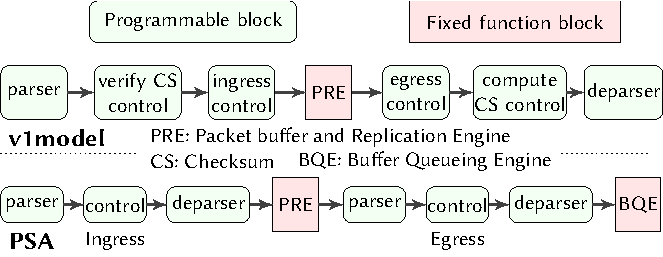
\includegraphics[width=\linewidth]{example-arch.pdf}
  \caption{Dataplane pipelines for example architectures}
  \label{fig:arch-example}
\end{figure}

To program a target, one can use P4 to specify the behavior of the
programmable blocks exposed in the architecture of the target. While
this approach allows supporting multiple targets which share the same
architecture, it also makes the P4 program dependent on
\begin{enumerate*}[label=(\roman*)]
  \item the target's dataplane pipeline,
  \item flow of packet and metadata in the pipeline, and
  \item target-specific constructs.
\end{enumerate*}
These dependencies pose multiple challenges for target-agnostic reuse
of independently developed P4 programs to build new ones:


% NOTE: Two main points:
% 1) across architectures: because pipeline model is different, it
% hinders portability and code reuse
% 2) even on the same architecture, a P4 program consists of
% sub-languages with different abstract machines. So, modular
% composition of programs is not possible.
% NOTE: introduce terms such as "abstract machine" with definition or
% examples

% First explain the problem with reuse across architectures
% (Portability)
\tightparbf{Challenge 1. P4 programs are specific to an architecture.}%
The structure of a P4 program is often dependent on the dataplane
pipeline model of the architecture for which it was written.
Architectures differ in the set of programmable-blocks and their
arrangement in the pipeline. So, when trying to reuse a program for
another target, if the architecture changes, it is often impossible to
reuse the same program with the new architecture without a complete
rewrite. For example, in \cref{fig:arch-example}, mapping the
functionality implemented for PSA's ingress deparser block to any
programmable block in \texttt{v1model}'s pipeline requires semantic
understanding of the blocks. Therefore, other than a manual rewrite,
there is no obvious automatic way to reuse the implementation of
programmable blocks across architectures.

Moreover, P4 programs often rely heavily on architecture-specific
metadata and constructs, such as resubmit, recirculate, clone,
etc.~\cite{simple_switch.md,psa}.  While this enables enable special
processing, such as replication, of packets, such dependency makes a
program tied to a specific architecture and undermines the program's
portability.

% (... and modularity)
\tightparbf{Challenge 2. P4 programs are monolithic.}
% TODO:
% Add some at least one direct reference to point 2 ``flow of packet 
% and metadata``. pieces of programs can be thought of many  ways.
% we have already mentioned about 'specifying behavior of 
% programmable blocks'. Another word pieces is confusing.
\refine{P4's programming model introduces unnecessary tight coupling 
among
pieces of the program which could be kept independent.} For example, 
in
\cref{fig:arch-example}, PSA's ingress parser initializes headers and
metadata which are processed by ingress control. To reuse the code for
ingress control block in another PSA-specific program, the new parser
must adhere to the headers and metadata generated by the previous
parser. Such coupling also manifests when trying to write modules for
otherwise independent packet-processing functions. This occurs because
P4 programs, often, use intrinsic and other metadata across a program
in an unrestricted manner~\cite{switch.p4}; it is difficult to split
such a program into clean modules which can be developed independently
and reused. More fundamentally, it breaks the notion of abstraction
needed to write modular programs. In fact, P4 does not enforce
sufficient scoping of data needed to develop independent modules. As a
result, even to update a small piece of functionality, developers need
to be aware of how each variable is used throughout the entire
program. Thus, tight coupling across program blocks and a lack of
proper scoping of data leads to monolithic programs, which makes it
extremely difficult to develop independent modules, thereby inhibiting
modularity.



% Then problem with writing modular code even on a single architecture
% (Composition)
\tightparbf{Challenge 3: Programmable blocks have heterogeneous
abstract machines.}%
The current approach also makes it hard to write composable dataplane
modules. To understand why, note that even for a fixed target, the
architecture usually contains packet-processing blocks with
heterogeneous execution models, also called \emph{abstract
machines}~\cite{p4lang,van1991machine}. For example in
\cref{fig:arch-example}, the parser blocks are described using a
sub-language of P4 which uses Finite State Machines (FSM) as its
abstract machine, while the control blocks are expressed in another
sub-language whose abstract machine models imperative control
flow~\cite{p4lang}. As the behavior of programmable blocks are
expressed in different sub-languages and abstract machines, a P4
program lacks a uniform or compatible interface between
packet-processing modules. This prevents modules to be composed
together to build larger programs. Going back to the earlier example,
in \cref{fig:ether.p4,fig:ipv4.p4}, ideally we would like to execute the
\texttt{ipv4} module (parser and control blocks) right before applying
\texttt{forward\_tbl} in \texttt{ether}'s \texttt{Pipe} control block so
that \texttt{nh\_id} is available in \texttt{forward\_tbl}. But the
existing P4 model does not support such composition.

% \hs{May be we can get away with summary and put shorter summary}
\deleted{
To summarize, there are three main challenges with current dataplane
programming model that hinders code portability, modularity and
composition:
\begin{enumerate}
  \item \hse{P4 programs are architecture-specific.}
    Different architectures vary in their dataplane pipeline model
    which have incompatible structure and semantics.  This renders P4
    programs written for one architecture not amenable to be ported to
    others.
  \item Architectures do not provide a clean abstraction that can
    decouple dataplane programs from targets and also do not enforce
    sufficient encapsulation and scoping of information. This makes it
    difficult to develop clean and independent modules.
  \item Programmable blocks within an architecture use heterogeneous
    abstract machines without a common interface. The lack of a
    compatible interface restricts composition of dataplane modules.
\end{enumerate}
}

To summarize, dataplane programs currently written in P4 are
\begin{enumerate*}[label=(\roman*)]
  \item not portable because of their affinity to architectures,
  \item monolithic because of huge data-sharing across
    processing-blocks within the pipeline and lack of scoping, and
  \item not composable because of heterogeneous abstract machines
    in processing-blocks and the lack of a uniform interface.
\end{enumerate*}




\subsection{Design goals and key insights}
\label{sec:goals}
\label{sec:insights}

Our main goal is to enable dataplane programming in a portable,
modular, and composable manner.

\tightpar{Portable:} Dataplane programs written for one target device
and architecture should be easily reusable across other targets and
architectures. For example, one should be able to port a program
originally written with \texttt{v1model} in mind on to PSA without
significant rewrite.

\tightpar{Modular:} Individual dataplane functionality for processing
packets can be developed in an independent manner agnostic of the
target as well as other dataplane functions. For example, one should
be able to write modules for Etheernet and IPv4 processing in an independent
manner.

\tightpar{Composable:} Modules for individual dataplane functions can
be composed together in custom ways to express complex dataplane
processing. For example, in \cref{fig:ether.p4,fig:ipv4.p4}, one should
be able to compose \texttt{ipv4} with \texttt{ether}, or replace
\texttt{ipv4} with modules for IPv6, MPLS etc. as needed.





\paragraph{Insights.}
We find that the root cause that restricts dataplane programming from
achieving our goals is the abstraction offered by current
architectures as discussed in~\cref{sec:challenges}.  Consequently,
our key insight is that in order to achieve the above goals, we need
% TODO:
% the generl term is misleading and confusing. We want to say in 
% clear words that out insigt is packet-processing abstractions based 
% on parser + MAT primitives are not enough, and we need abstraction 
% for entire dataplane 
\refine{\emph{to raise the level of abstraction that is general 
enough to
  express a wide range of functionality while also being realistic so
  that programs can be mapped to real architectures in an automatic
manner}}. Of course, introducing yet another architecture to unify
existing architectures would add significant complexity to the
ecosystem; instead, what we need is a \emph{logical} architecture that
acts as high-level description against which programs are written, and
this logical architecture maps to real architectures. This
architecture is logical in the sense that devices do not explicitly
implement it; rather, it captures the bare essence of packet
processing and exposes that to programs.

Based on our analysis in \cref{sec:challenges}, we found that the
challenges stem from inconsistent pipelines across architectures,
exposing target-specific externs, and a lack of uniform abstract
machine and interfaces with any existing architecture. Accordingly, we
believe that the logical architecture should have three main
components:
\begin{enumerate*}[label=(\roman*)]
  \item a logical pipeline that is expressive enough to encode a
    wide range of packet-processing functions while being general,
  \item a generic way to use target-specific features such as externs
    without introducing tight coupling, and
  \item a common interface so that packet-processing modules can be
    composed.
\end{enumerate*}


\subsection{Overview of our approach}
\label{sec:overview}
%% Give an overview of our approach, tying to the above discussion
%% Do not go into specific details yet.

To achieve our goals of portable, modular and composable dataplane
programming without disrupting the existing workflow for P4, we
introduce the \ulang framework. \ulang implements the above insights
using two main components:
\begin{enumerate*}[label=(\roman*)]
  \item \uarch: an architecture for an intermediate logical device
    called \uswitch (\cref{sec:architecture}) and
  \item \ucomp: a compiler that translates \ulang programs into real
    target code (\cref{sec:compiler}).
\end{enumerate*}

Users write dataplane programs using an extended P4 language which
supports modularity and composition. These programs are written with
the \uarch architecture. While compiling, users specify the real
target architecture for which the \ulang programs should be
translated. This decouples programs from target architectures while
keeping the workflow very simple and intuitive.

\uarch raises the dataplane programming abstraction from
target-specific pipelines in a way that enables writing modular code
with a common interface that hides implementation details. A module
receives a complete or partial packet along with certain metadata,
processes it as needed, and sends out one or more packets along with
metadata. Thus, each module can be developed independently. Modules
communicate with each other through a well-defined compatible
interface---a logical buffer introduced by \uswitch.  With this,
\uswitch abstracts away the details of dataplane pipelines of real
targets. To express special processing, such as packet replication, in
\ulang modules, \uarch introduces \emph{logical externs}.

\ucomp compiles \ulang programs for a specified target while
conforming to the constraints of the target device in two main steps.
First, \ucomp compiles the program to a \uarch-specific Intermediate
Representation (IR). It homogenizes the abstract machine for each
block by transforming all programmable blocks into match-action units.
This enables natural transfer of execution-control across modules, as
well as code reuse and composition. In the second step, \ucomp
translates the IR into a configuration specific to the target.

\deleted{The logical pipeline models defined in \uarch do not completely
eliminate heterogeneity in packet-processing blocks (parser,
control) of the pipelines.
% However, constructs and pipeline models declared in \uarch allows to
% write programs by reusing the code developed in conformance of
% \uarch.
The design choices for \uarch are intentional to avoid disruptive
innovations in P4 language.  It partially address the above mentioned
challenges and leaves following two aspects for unaddressed.  $1$
creating P4 programs specific to \uarch and the logical device \ucomp.
$2$ heterogeneity in packet-processing blocks of P4 programs.  We
complement design choices of \uarch by designing and developing a
compiler, \ucomp, to address these aspects.
}



%%%%%%%%%%%%%%%%%%%%%%%%%%%%%%%%%%%%%%%%%%%%%%%%%%%%%%%%%%%%%%%%%%%%%%
%%%%% MICRO-P4 %%%%%%%%%%%%%%%%%%%%%%%%%%%%%%%%%%%%%%%%%%%%%%%%%%%%%%%
%%%%%%%%%%%%%%%%%%%%%%%%%%%%%%%%%%%%%%%%%%%%%%%%%%%%%%%%%%%%%%%%%%%%%%
\section{The \ulang framework}
\label{sec:microp4}
%% Describe each component of microP4
Now, we describe each component of \ulang to show how \ulang achieves
our goals for dataplane programming.
\begin{figure}[!tb]
    \centering
    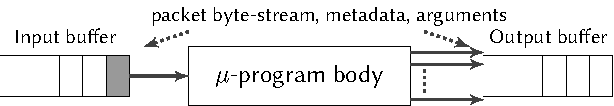
\includegraphics[width=\linewidth]{uswitch-model}
    \caption{Abstract programming model for \uswitch}
    \label{fig:uswitch}
\end{figure}


\paragraph{\uswitch.}
\uswitch is an intermediate logical target with an abstract
programming model. It is designed to provide a high-level dataplane
abstraction that enables modular programming without compromising
expressiveness to process packets. It does so by allowing to write
modules that implement fine-grained packet processing and defining
interfaces to compose these modules.

\uswitch models each packet-processing module as a self-contained
execution unit, called a \emph{\uprogram}, and executes it using the
model shown in \cref{fig:uswitch}. A \uprogram takes as input: a
packet byte-stream, metadata and arguments for user-defined
parameters. As output, it generates byte-streams, metadata, and return
values corresponding to one or more packets. Such a model hides
implementation details---such as header types, local state,
user-defined metadata and match-action tables---of a \uprogram from
other \uprograms.  \uswitch fetches an element from a logical input
buffer for each \uprogram, executes the \uprogram and writes one or
more elements to the logical output buffer, which acts as input for
another. Note that these buffers exist only in the abstraction and do
not represent buffers in real target devices.

\paragraph{\uswitch Architecture (\uarch).}
To write portable \uprograms, we define \uswitch Architecture
(\uarch)---it specifies the dataplane as composition of logical
pipelines, called \emph{\upipeline}, where each \upipeline implements
a part of the complete packet processing on the device. A \upipeline
may map to one or more \uprograms. Each \upipeline is associated with
a \uarch interface which specifies run-time parameters in a generic
way and declares programmable blocks required to be implemented for
the pipeline. In order to capture the fundamentals of
packet-processing and expose a minimal interface, \upipelines comprise
of only programmable blocks such as parser,
match-action control and deparser. In addition, to abstract
away from target-specific constructs, \uarch provides \emph{logical}
externs and metadata to facilitate use of packet-processing features
such as multicast, cloning, etc. that are not part of the core P4
language but supported by actual target devices.

\begin{figure}[!tbp]
  \begin{subfigure}{\linewidth}
    \centering
    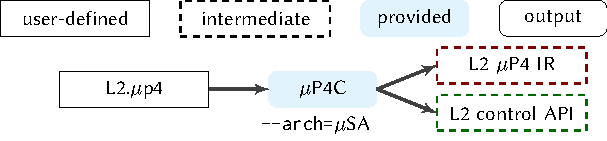
\includegraphics[width=\linewidth]{compilation-module.pdf}
    \caption{Compiling a \ulang module into IR.}
    \label{fig:compile-module}
  \end{subfigure}
  \begin{subfigure}{\linewidth}
    \centering
    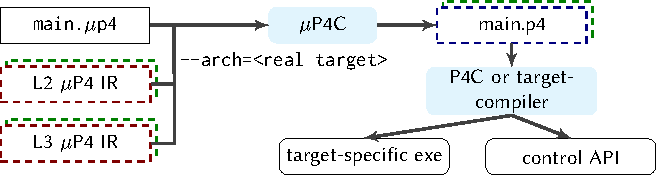
\includegraphics[width=\linewidth]{compilation-main.pdf}
    \caption{Compiling a \ulang program with other modules for a
    target.}
    \label{fig:compile-to-target}
  \end{subfigure}
  \caption{Compiling \uprograms}
  \label{fig:compiler-workflow}
\end{figure}

\paragraph{\ulang and Compiler (\ucomp).}%
\ulang extends P4 and allows users to write libraries of independent
packet-processing modules, declare their instances and invoke the
instances using a built-in \texttt{apply} method. This allows to hide
implementation of a module and reuse them using run-time parameters of
their interfaces. Note that \ulang programs are written in a
target-agnostic manner using logical constructs of \uarch. To use
\ulang for a given target device, we need to generate configurations
specific for that target. For this, we present the \ulang compiler,
\ucomp.

\cref{fig:compiler-workflow} gives an example of building a dataplane
with \ulang and \ucomp in two stages:
\begin{enumerate*}[label=(\roman*)]
  \item compiling individual modules and
  \item composing modules and compiling dataplane for a target.
\end{enumerate*}
Users write individual modules for specific processing---for example,
\texttt{ether.\ulang} in \cref{fig:compile-module} performs only
ethernet processing similar to \cref{fig:ether.p4}.
\cref{fig:compile-module} shows the first stage of compiling where
\ucomp compiles a module into \uarch-specific IR.   In the second
phase, users can link different modules together to build a
dataplane---e.g., in \cref{fig:compile-to-target},
\texttt{main.\ulang} composes Ethernet and IPv4 modules to build a
modular router. During this, \ucomp transforms parser and deparser
blocks of each module into match-action control. This transformation
unifies the abstract-machines for packet-processing, thus allowing
seamless transfer of execution control within and across modules and
enables composition. Further, based on the specified target device,
the compiler also generates the dataplane configuration specific to
the device through a sequence of intermediate steps
(\cref{sec:compiler}).


% \deleted{
% \ulang extends P4 and allows programmers to define \texttt{package}
% types, declare their instances and invoke them using the built-in
% \texttt{apply} method. This allows to hide implementation of package
% types and reuse them using run-time parameters of their interfaces.
% Programmers can use sub-languages of P4 for parser and control blocks
% to implement interfaces.  \ucomp homogenizes abstract-machines of
% programmable blocks by transforming parser and deparser blocks into
% match-action control blocks.
% Each \uprogram specializes a generic interface. The run-time 
% interfaces enable easy reuse and hide implementation detail of the 
% \uprograms, facilitating modular and incremental development. Using 
% logical data plane model of \uarch, programmers can develop modular 
% P4 code which is specific to \uarch. We design and develop MicroP4 
% Compiler (\ucomp) to compile and transform \uprogram for 
% architectures of real target devices, making \uprograms agnostic of 
% architectures of real-targets. Programmer can use \ucomp to $(1)$ 
% Create compiled libraries of \uprograms along with their control 
% plane APIs, $(2)$ Link all the \uprograms used in the \uprogram of 
% main instance and transform the program for a specified architecture 
% of a real-target.
% If the given source file does not contain an instance named, \ucomp 
% generates a library by compiling it to an Intermediate Representation 
% (IR) in json format (Figure \ref{subfig:module-compilation}). It also 
% generates architecture-independent control-plane APIs, P4Runtime 
% \cite{p4runtime} files. If the source file contains \emph{main} 
% instance, it links all the supplied libraries and transforms the 
% \uprogram of main instance for a given architecture (Figure 
% \ref{subfig:compilation-to-target-architecture}). Programmers can 
% include files containing definitions of data types (e.g., struct 
% types 
% of in and out parameters) used in run-time interfaces of \uprogram in 
% libraries. \ucomp compiler generates either source P4 code for the 
% specified architecture or an executable with architecture-specific CP 
% APIs.
% }

% \deleted{\ucomp perform static analysis to estimate possible packet 
% sizes required to process all the transformed \uprograms in 
% match-action control blocks of target architecture's pipeline.
% \ucomp synthesizes P4 code for parser and deparer blocks of target architecture's pipeline to extract and emit required number of bytes from and to packet.
% It allocates and schedules code of transformed \uprograms to control 
% blocks of the target architecture's pipeline model while satisfying 
% constraints posed by hardware details.}






%%%%%%%%%%%%%%%%%%%%%%%%%%%%%%%%%%%%%%%%%%%%%%%%%%%%%%%%%%%%%%%%%%%%%%
%%%%% Micro Switch Architecture %%%%%%%%%%%%%%%%%%%%%%%%%%%%%%%%%%%%%%
%%%%%%%%%%%%%%%%%%%%%%%%%%%%%%%%%%%%%%%%%%%%%%%%%%%%%%%%%%%%%%%%%%%%%%
\section{\uswitch Architecture (\uarch)}
\label{sec:architecture}
In this section, we describe \uarch using two main constructs:
\begin{enumerate*}[label=(\roman*)]
  \item \emph{\upipelines} and interfaces for writing \ulang programs
    (\cref{sec:pipelines}) and
  \item \emph{logical externs} for expressing special processing of
    packets in a target-agnostic manner (\cref{sec:logical-externs}).
\end{enumerate*}


\subsection{\upipelines and Interfaces}
\label{sec:pipelines}

\tightpar{\upipeline.}%
\uarch models the dataplane as composed of two types of \upipelines:
\emph{linear} and \emph{orchestration} as shown in
\cref{fig:pipe-types}. A linear \upipeline models processing a single
input packet through a linear set of stages: parser, match-action
control, and deparser.  As output, it may generate multiple packets
for a single input, but each packet is processed by the same code. In
contrast, an orchestration \upipeline can process multiple copies of a
packet in different user-defined ways. A combination of these
\upipelines enables expressing a wide range of packet-processing
behavior.
\begin{figure}[!tbp]
  \centering
  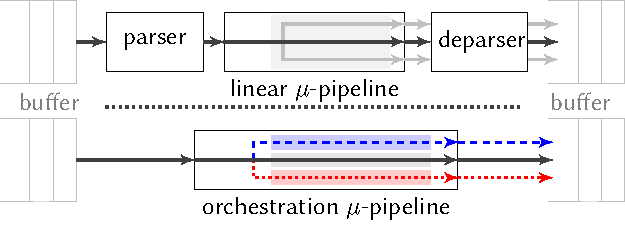
\includegraphics[width=0.8\linewidth]{upipe-types}
  \caption{Types of \uarch pipelines: linear and orchestration}
  \label{fig:pipe-types}
\end{figure}

\tightpar{Interfaces.}%
To build a \uprogram by composing \upipelines, \uarch provides three
types of interfaces: \texttt{Unicast}, \texttt{Multicast} and
\texttt{Orchestration}.  \texttt{Unicast} and \texttt{Multicast} are
used by linear \upipelines, while \texttt{Orchestration} is used by
orchestration \upipelines. These interfaces specialize the logical
buffers that pipelines use for input and output
(\cref{fig:pipe-types})---e.g., a linear \upipeline that writes
multiple packets may use a \texttt{Multicast} interface to specialize
its output buffer. Implementing interfaces for each \upipeline in a
\uprogram also automatically declares the run-time interface for the
\uprogram---this is useful for composing \uprograms.

The following snippet shows the signature of these interfaces while
\cref{fig:micro-switch-architecture} shows declarations of
types---such as \texttt{pkt}, \texttt{sm\_t}, etc.---used in the
signature and \cref{fig:modular-router} shows an example of using the
\texttt{Unicast} interface.

\begin{lstlisting}[frame=none]
Unicast<I,O,IO> (pkt p, im_t im, in I i_param, out O o_param, inout IO io_param);
Multicast<I,O> (pkt p, im_t im, in I i_param, out_buf<O> ob);
Orchestration<I,O> (in_buf<I> ib, out_buf<O> ob);
\end{lstlisting}

To implement the model shown in \cref{fig:uswitch}, \uswitch
implicitly performs a few operations while invoking 
\uprograms---e.g., note that \texttt{Unicast}'s signature does not 
have any
buffer in its parameters, while \texttt{Orchestration} needs two
buffers as arguments. So, \uswitch fetches an element from an implicit
logical input buffer for \uprograms with \texttt{Unicast} or
\texttt{Multicast} interface, while for \uprograms with
\texttt{Orchestration} interface, it fetches the elements from the
specified input buffer.


% \uarch allows programmers to write multiple implementations of 
% the same interface type to define multiple \upackages with 
% required run-time behaviors.
% Micro pipeline comprises of a parser, a control and a deparser 
% block.\uarch does not allow conditional statements in deparser 
% blocks of its % pipelines.
% For each pipeline type, it exposes one or more interface types.
% Each interface type comprises of a set of declarations for 
% programmable blocks and runtime signature.
% Programmers can provide implementations of the interface types 
% to create user-defined P4 package types.
% To implement an interface type, programmers need to implement 
% all the programmable blocks of the interface type.
% Programmers can instantiate variable of user-defined package 
% types and invoke the instances using built-in  \texttt{apply} 
% method similar to control blocks.
% The \texttt{apply} method of package instance can be called by 
% supplying arguments for run-time parameters of the interface 
% implemented by the package type.
% Every incoming packet is parsed and validated by the parser, if 
% parser terminates in \texttt{accept} state, then execution 
% control is transferred to micro control block.
% If the execution control reaches till the end of the micro 
% control block, packet is processed by the deparser block.
% Orchestration pipeline has only a control block, named 
% orchestration.
% Programmers can implement programmable blocks of Micro pipeline 
% to create custom package types having runtime signature same as 
% unicast 
% or multicast interface.
% Similarly, Orchestration interface is associated with 
% Orchestration pipeline.

% /* standard metadata */
% struct sm_t { 
%   bit<16> pkt_len;
%   bit<8> in_port;
% }


\begin{figure*}
\begin{minipage}[t]{.38\textwidth}
\begin{lstlisting}[frame=none]
extern pkt { /* packet representation */
  byte[] packet; 
  unsigned length;
  void copy_from(pkt pa);
}
extern emitter { /* packet assembler */
  void emit<H>(pkt p, in H hdr);
}
\end{lstlisting}
\end{minipage}\vline
\hfill
\begin{minipage}[t]{.24\textwidth}
\begin{lstlisting}[frame=none]
/* enum to map to target-specific metadata */
enum meta_t {
  IN_TIMESTAMP,
  OUT_TIMESTAMP,
  IN_PORT, PKT_LEN,
  ...
}
\end{lstlisting}
\end{minipage}\vline
\hfill\begin{minipage}[t]{.35\textwidth}
\begin{lstlisting}[frame=none]
/* Multicast extern object*/
extern mc_engine {
  mc_engine();
  void set_mc_group(GroupId_t gid);
  apply(im_t, out PktInstId_t);
  set_buf(out_buf<O>);
  apply(pkt, im_t, out O);  
}
\end{lstlisting}
\end{minipage}
\begin{minipage}[t]{0.47\textwidth}
\begin{lstlisting}[frame=none]
extern extractor { /* Data Extraction */
  void extract<H>(pkt p, out H hdr);
  void extract<H>(pkt p, out H hdr, in bit<32> size);
  H lookahead<H>();
}
extern im_t {/* Correlated intrinsic metadata */
  void set_out_port(in bit<8>);
  bit<8> get_out_port();
  bit<32> get_value(in meta_t ft);
  void copy_from(im_t im);
}
\end{lstlisting}
\end{minipage}\vline
\hfill\noindent\begin{minipage}[t]{0.52\textwidth}
\begin{lstlisting}[frame=none]
extern in_buf<I> { // used only by architecture
  dequeue(pkt, im_t, out I);
}
extern out_buf<O> {
  enqueue(pkt p, im_t im, in O out_args);
  void to_in_buf(in_buf<O>);
  void merge(out_buf<O>);
}
extern mc_buf<H, O> {
  enqueue(pkt, in H, im_t, in O);
}
extern void recirculate<D>(in D data);
\end{lstlisting}
\end{minipage}
\caption{Declarations in Micro-Switch Architecture}
\label{fig:micro-switch-architecture}
\end{figure*}



\subsection{Logical Externs}
\label{sec:logical-externs}
\uarch's logical externs  enable representing packets and metadata as
well as expressing packet-processing functions in a target-agnostic
manner. These generic constructs, shown in
\cref{fig:micro-switch-architecture}, are mapped to target-specific
constructs eventually.

\tightparbf{Packet Extern.}
\uarch allows representing a packet as a byte-array through an extern
called \texttt{pkt}. Users can also instantiate and initialize new
\texttt{pkt} instances using \texttt{copy\_from} method.  To allow
modifications on a \texttt{pkt} instance, \uarch's provides the
\texttt{extractor} and \texttt{emitter} externs.
% While a \texttt{pkt} needs to be initialized, \texttt{emitter}
% and \texttt{extractor} do not need to be initialized.

% The \texttt{pkt} instance, in parameters of every processing-block, is
% supplied by \uswitch. Also, \uswitch allows to create compile-time
% copies of packets by declaring \texttt{pkt} instances and initializing
% them using the \texttt{copy\_from} method in implementation of the
% control block of only the orchestration pipeline.

% The \texttt{copy\_from} method initializes its caller instance with 
% content of \texttt{pa} without modifying the argument.
% \uswitch considers this method as a compile-time known packet 
% replication, whereas multicast as a runtime packet-replication.
% To extract and insert data in \texttt{pkt}, \uarch provides two 
% externs objects, \texttt{extractor} and \texttt{emitter}.
% The \texttt{extractor} and \texttt{emitter} externs can not be 
% instantiated, their instances are provided by the \uswitch as 
% parameters in parser and deparser declarations of \texttt{Unicast} 
% and \texttt{Multicast} interfaces. 

\tightparbf{Intrinsic Metadata and Constraints.}
Architectures of actual targets usually provide intrinsic per-packet
metadata with certain constraints on their usage---e.g.,
\texttt{output\_port} cannot be changed in the PSA's egress pipeline
to meet the packet scheduler's requirements~\cite{psa}.

To use such metadata and also to capture any constraints, \uarch
provides an extern, \texttt{im\_t}, and an enumerator,
\texttt{meta\_t}. \texttt{meta\_t} maps \uarch's metadata to
target-specific metadata---each value in the enumerator maps to an
immutable intrinsic metadata field specific to the target, for
example, \texttt{ingress\_timestamp}. Note that \texttt{meta\_t} needs
to be defined for each target architecture in \ucomp's backend
(\cref{sec:compiler}), which also enforces any constraints on
metadata. To access a metadata's value, set by the target, in a
program, \texttt{im\_t} provides a method \texttt{get\_value}, which
is parameterized on \texttt{meta\_t}.
% The extern exposes methods to access correlated intrinsic metadata. 
% For example \texttt{set\_out\_port} and \texttt{get\_out\_port} 
% allow, respectively, sets and gets output port for the packet.
% \uarch defines intrinsic metadata for the logical target \uswitch.
% For every real-target architecture , \ucomp maintains mapping of 
% its 
% logical intrinsic metadata with the metadata of the architecture.
% This mapping is used for transforming \uprograms to a given 
% architecture-specific code.
% 
% 
% 
%  The first parameter with \texttt{in} direction is of 
% \texttt{meta\_t} type indicating a particular metadata field. The 
% second parameter with \texttt{out} direction provides value of the 
% field.
% \ucomp allows repeated usage of the extern's functions in the 
% single 
% control block of \uarch pipelines.
% If \emph{get\_value} occurs before \emph{set\_egress\_port} on any 
% possible execution control path, \ucomp raises a compile-time 
% error.



\begin{figure*}[!ht]
\noindent \begin{minipage}[t]{.50\textwidth}
\begin{lstlisting}[frame=none, escapechar=!]
/* !{l3.\ulang}! */
// !{\color{commentcolor}{\uprograms for L3 protocols}}! 
ipv6(pkt p, im_t im, out bit<16> nh_id);
ipv4(pkt p, im_t im, out bit<16> nh_id);
// implement unicast interface for L3 program
!\colorbox{green!10}{program L3 : implements Unicast<>}! {
  parser P(extractor ex, pkt p, out empty_ht h, inout data_t d) {
    state start { transition accept; }
  }
  control C(pkt p, inout empty_ht h, im_t im,
      out bit<16> !\colorbox{mygray}{nh\_id}!, inout bit<16> !\colorbox{mygray}{type}!) {
    ipv4() !\colorbox{red!10}{ipv4\_i}!; ipv6() !\colorbox{red!10}{ipv6\_i}!; // instantiation
    apply { switch (!\colorbox{mygray}{type}!) { // out arg: nh_id
        0x0800:!\colorbox{red!10}{ipv4\_i}!.apply(p, im, !\colorbox{mygray}{nh\_id}!);
        0x86DD:!\colorbox{red!10}{ipv6\_i}!.apply(p, im, !\colorbox{mygray}{nh\_id}!);
    } }
  }
  control D(emitter em, pkt p, in empty_ht h) {
    apply { }
  }
}    // L3 program sets the next hop (nh_id)
!{\subcaption[]{l3.\ulang implements IPv4 and IPv6}\label{subfig:router}}!
/* !{modular\_router.\ulang}! uses L3 program */
!\colorbox{green!10}{L3}!(pkt p, im_t im, 
out bit<16> !\colorbox{mygray}{nh\_id}!, inout bit<16> !\colorbox{mygray}{type}!);
\end{lstlisting}
\end{minipage}\hspace{-4pt}\vline
\hfill\begin{minipage}[t]{.50\textwidth}
\begin{lstlisting}[frame=none, escapechar=!]
!\colorbox{green!10}{program ModularRouter : implements Unicast<>}! {
parser P(extractor ex, pkt p, out hdr_t h) {
  state start {
    ex.extract(p, h.eth); transition accept;
  }
}
control C(pkt p, inout hdr_t h, im_t im) { // p is partial pkt without L2 header
  bit<16> !\colorbox{mygray}{nh\_id;}! !\colorbox{green!10}{L3()}! !\colorbox{red!10}{l3\_i; }!
  action drop () {}
  action forward(bit<48> dmac, bit<48> smac, bit<8> port) {
    h.eth.dstMac = dmac; h.eth.srcMac = smac;
    !\colorbox{blue!10}{es}!.set_out_port(port); // setting metadata
  }
  table forward_tbl { // L2 forwarding, needs nh_id
    key = { nh_id : exact; } 
    actions = { forward; drop; }
  }
  apply { // invoke L3 to get nh_id
    !\colorbox{red!10}{l3\_i}!.apply(p, im, !\colorbox{mygray}{nh\_id}!, !\colorbox{mygray}{h.eth.etherType}!);
    forward_tbl.apply(); // use nh_id in forward_tbl
  }
}
control D(emitter em, pkt p, in hdr_t h) {
  apply { em.emit(p, h.eth); }
}
}
ModularRouter(P, C, D) main;
\end{lstlisting}
% 0x8847:!\colorbox{mygray}{mpls\_i.apply(p, sm, es);}!
\subcaption[]{Modular Router \uprogram composes L2 and L3 routing.}\label{subfig:router-main}
\end{minipage}
\caption[]{Modular Router using \uarch \footnotemark}
\label{fig:modular-router}
\end{figure*}
\footnotetext{For brevity, we have skipped the unused parameters in 
parser, control blocks and declarations of \uprograms.}


% We illustrate modular programming and composition using the logical 
% constructs introduced till now.

\tightpar{Example: Modular router using \texttt{Unicast} interface and
externs.}
\cref{subfig:router} shows a program, \texttt{l3.\ulang}, that
implements the \texttt{Unicast} interface and processes IPv4 and IPv6
headers.\footnotemark[\value{footnote}] Both \texttt{ipv4} and
\texttt{ipv6} declare a user-defined parameter, \texttt{nh\_id} as a
part of run-time parameters along with packet \texttt{p} and intrinsic
metadata \texttt{im}. Similarly, \texttt{L3} exposes another
parameter, \texttt{type}.  Such user-defined parameters allow flexible
passing of data across modules for composition.

\texttt{ModularRouter}, in \cref{subfig:router-main}, parses the
ethernet header and invokes an instance of L3, by calling
\texttt{l3\_i.apply()}. It passes a partial packet `\texttt{p}',
without the ethernet header, to \texttt{L3}.  \texttt{L3}, in turn,
uses the \texttt{type} argument to invoke an instance of the
appropriate protocol---IPv4 or IPv6---which populates \texttt{nh\_id} 
passed as an \texttt{out} argument. \texttt{ModularRouter}
uses the value of \texttt{nh\_id} and continues processing by
applying \texttt{forward\_tbl}.







\tightparbf{Multicast Extern.}
To express programs that need packet replication, \uarch provides the
\texttt{mc\_engine} extern. It can be instantiated inside a control
block while implementing the \texttt{Multicast} interface as shown in
the listing in \cref{app:multicast}.  To store copies of parsed
headers, unparsed packet, metadata and other data related to a packet,
\texttt{Multicast} provides a buffer (of type \texttt{mc\_buf},
explained next) as one of the parameters.  Users can create copies of
a packet by invoking \texttt{mc\_engine}'s \texttt{apply} method.
Logically, this can be thought of as spawning multiple \upipelines,
each processing one packet replica, according to specified
configurations. In each \upipeline, all reachable statements from the
call are executed.
For a detailed description of other methods, see \cref{app:multicast}.

% For example, had \texttt{ipv4} and 
% \texttt{ipv6} implemented using multicast interface, the 
% \texttt{forward} table in the \texttt{Router} \uprogram have to be 
% applied on all the copies of partial packet.
% The caller (\texttt{Router}) can cascade multicast processing on 
% partial packets. It can $(1)$ store the partial copies, generated 
% by 
% the callee, into an instance of \texttt{mc\_engine} using 
% \texttt{set\_buf} and $(2)$ invoke the apply method to process each 
% copy using subsequent statments). 




\paragraph{Input/Output Buffers.}
Corresponding to the logical buffers in \uswitch's model
(\cref{fig:uswitch}), \uarch declares \texttt{in\_buf} and
\texttt{out\_buf} externs. These are used to invoke other programs
from within the control block of an \texttt{Orchestration} \upipeline.
As \uswitch restricts fetching multiple packets simultaneously
from the input buffer, \texttt{in\_buf}'s \texttt{dequeue} method
can be used only  the \uswitch. However, programmers can use them to
pass as arguments to other modules. \texttt{out\_buf} exposes
\texttt{enqueue} and \texttt{merge} methods to buffer packets
processed by the callee program. to move elements to an
\texttt{in\_buf} instance, which is passed as the argument, users
can use \texttt{to\_in\_buf}. Unlike \texttt{in\_buf} and
\texttt{out\_buf}, the \texttt{mc\_buf} extern allows to store 
replicated parsed headers for multicast.
\deleted{
It is designed to be used along with
\texttt{mc\_engine} to express multicast packet-processing, where as
\texttt{in\_buf} and \texttt{out\_buf} are designed for generic
composition interface.
}

% \begin{figure}[htb]
% \begin{lstlisting}[frame=none, escapechar=!]
% control mc(pkt p, hdr_t h, sm_t s, es_t e, 
% !\colorbox{mygray}{mc\_buf<hdr\_t, out\_t> hb}!) {
%   !\colorbox{mygray}{mc\_engine mce;}!  PktInstId_t id; 
%   !\colorbox{mygray}{out\_t oa;}! // some out args
%   action replicate(GroupId_t gid) {
%     !\colorbox{mygray}{mce.set\_mc\_group(gid);}!
%   }
%   table MulticastRouting{ key = { ... } 
%     actions = { replicate; }
%   }
%   table mac{ ...}
%   apply {
%     MulticastRouting.apply();
%     !\colorbox{mygray}{mce.apply(es, id);}!//similar to C's fork
%     mac.apply();
%     !\colorbox{mygray}{hb.enqueue(h,  es, oa);}!
%   }
% }
% \end{lstlisting}
% \caption{Multicast Example}
% \label{fig:multicast-example}
% \end{figure}



















%%%%%%%%%%%%%%%%%%%%%%%%%%%%%%%%%%%%%%%%%%%%%%%%%%%%%%%%%%%%%%%%%%%%%%
%%%%% MICRO P4 Compiler %%%%%%%%%%%%%%%%%%%%%%%%%%%%%%%%%%%%%%%%%%%%%%
%%%%%%%%%%%%%%%%%%%%%%%%%%%%%%%%%%%%%%%%%%%%%%%%%%%%%%%%%%%%%%%%%%%%%%
\section{\ulang Compiler (\ucomp)}
\label{sec:compiler}
In this section, we present the design of \ucomp--a compiler that
transforms target-agnostic \ulang programs to configurations for a
specified target architecture---with focus on key transformations that
enable composition.

\begin{figure*}[!tbh]
  \centering
  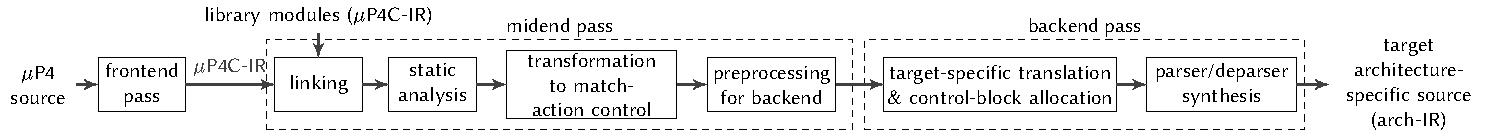
\includegraphics[width=\linewidth]{workflow}
  \caption{Overview of transformations performed in different phases
  in \ucomp: frontend, midend, and backend.}
  \label{fig:workflow}
\end{figure*}

\subsection{\ucomp Design Overview}
\label{sec:compiler-design}
\ucomp builds on the P4 reference compiler, \texttt{p4c}~\cite{p4c},
and has a modular design consisting of three phases: \emph{frontend},
\emph{midend} and \emph{backend}. \cref{fig:workflow} shows an
overview of \ucomp's phases.

\tightparbf{Frontend.}%
The frontend transforms \ulang programs into \ucomp-specific
intermediate representation (\ucomp-IR). It performs basic checks like
type-checking at the source-level. As output, it generates reusable
libraries by serializing the \ucomp-IR.

\tightparbf{Midend.}%
\ucomp's midend is responsible of two main transformations:
\begin{enumerate*}[label=(\roman*)]
  \item homogenizing processing blocks to enable composition and
  \item preprocessing for the backend pass.
\end{enumerate*}

To compose \uprograms by homogenizing their processing blocks, first,
it performs static analysis of the \uprogram to compute the
``operational-region''---i.e., the region of a packet's byte-stream
that the program needs to access. Then, it synthesizes a stack of
one-byte headers, called a \emph{byte-stack}, large enough to store
the operational-region. Finally, considering this byte-stack as a
packet, it transforms any (de)parsers into homogeneous match-action
control blocks.

To preprocess for the backend, in case of compile-time replication,
\ucomp's midend extracts packet-processing code for every packet
instance and prepares a processing schedule.

The midend passes are agnostic to target architectures, and focus on
composition and pre-processing for the backend passes. At the end of
the midend passes, the \ucomp-IR contains only control blocks having
\uarch-specific constructs.

\tightparbf{Backend.}%
\ucomp's backend, which is specific to a target architecture, has two
goals:
\begin{enumerate*}[label=(\roman*)]
  \item to translate and allocate control blocks to the target's
    dataplane pipeline while respecting any constraints on metadata
    and
  \item to synthesize any required parser and deparser blocks in
    the target's pipeline model.
\end{enumerate*}



\subsection{\ucomp Midend}
\label{sec:compiler-midend}
We present a brief overview of the transformation passes of the
midend. Then, we elaborate on only the crucial passes.

The midend begins with linking the \ucomp-IRs of all the \uprograms
that need to be composed to build the dataplane. Then, it performs
two transformations on every \uprogram:
\begin{enumerate*}[label=(\roman*)]
  \item convert each header-stack instance into a set of header
    instances and
  \item convert each \texttt{extract} method call that parses
    variable-length headers to a sub-parser that uses only
    fixed-length extractions to parse the header.
\end{enumerate*}
These transformations convert a parse graph into a Directed Acyclic
Graph (DAG), simplifying the \uprograms for the next pass.
% , which performs \emph{static analysis}.

\tightpar{Static analysis.} The simplified \uprograms allow computing
minimum and maximum bytes that are extracted by the parsers and
emitted by the deparsers. These values, in turn, are used to compute
the operational-region for the composed program and store it in a
byte-stack (\cref{subsubsection:static-analysis}).

Having a byte-stack storing packets' operational-regions allows to
synthesize a match-action table that can parse and deparse packets.
Following static analysis, the midend performs these transformations
on \ucomp-IR to homogenize all processing blocks to match-action
control blocks (\cref{subsection:parser-to-match-action-table}).
Naturally, the ``main'' \uprogram---i.e. the one composing together
different \uprograms---in \ucomp-IR is also transformed to a control
block that invokes others.

Finally, if the main \uprogram is dependent on a \uprogram that
implements the \texttt{Orchestration} interface, the final midend pass
extracts processing code for every packet instance created during
\texttt{Orchestration} in the \uprogram. In addition, it prepares an
execution schedule to capture interaction among processing of packet
instances.




% First, the midend replaces header stacks and variable-length header 
% with multiple instances of headers, creating parsers in all the 
% \uprogram without cycles and variable-length extraction.
% Next, it performs static-analysis to midend determine two important 
% metrics, $(1)$ the maximum number of bytes, called 
% \emph{extract-length}, to be extracted to execute the composed 
% \uprogram and $(2)$ the size of byte-stack required to hold the 
% extracted bytes and any new header instance that may be inserted into 
% the packet.
% Third, it transforms (de)parser blocks into match-action control 
% blocks.

% \ucomp transforms parsers and deparsers of the main and callee 
% package types into match-action control blocks.
% It synthesizes new parser and deparser for the main package.
% The synthesized parser accepts every packet with length greater than 
% the minimum length, called \emph{min-packet-size}, derived by 
% static-analysis of the program. For every accepted packet, the 
% synthesized parser at most extracts a fixed number, called 
% \emph{extract-length}, of bytes to a stack, called \emph{byte-stack}, 
% of one-byte headers. Programs may increase or decrease size of 
% packets, therefore, the estimated size of byte-stack can be greater 
% than extract-length. The synthesized deparser emits all valid 
% one-byte headers from the byte-stack.
% 
% We perform compile-time analysis of parser, control and deparser 
% blocks to estimate min-packet-size, extract-length and the size of 
% byte-stack to process packets, as explained in section 
% \ref{subsection:extract-length-and-byte-stack-size}. \ucomp executes 
% transformed parsers and deparsers in the match-action stages using the 
% byte-stack. For each program, \ucomp creates metadata variables, 
% called \texttt{field-variables} for the header fields used in the 
% program's control block. The header fields are substituted with the 
% metadata variables in control blocks of the program. \ucomp discards 
% types and instances of the headers of each package. \ucomp 
% synthesizes a single bit \emph{valid} metadata variable for each 
% header instance to record its presence in the packet. 
% \texttt{setValid} and \texttt{setInvalid} method-call statements of 
% every header instance is replaced with assignments on the related 
% \emph{valid} metadata variable. Execution of parsers in match-action 
% stages copy values from the appropriate locations in the byte-stack to 
% the variables. It also updates valid metadata variables which are 
% later used by the deparser to copy back field-variables to byte-stack.
%  
% 
% Section \ref{subsection:parser-to-match-action-table} discuss about 
% converting simple parser into a match-action table. Section 
% \ref{subsection:header-stacks-variable-length-headers} converts 
% parsers with header stacks or variable-length header into simple 
% parser}
 
% TODO: mention recursion at right place in limitations. We do not 
% allow it by compile-time check. 
\subsubsection{Static Analysis}
\label{subsubsection:static-analysis}
\ucomp performs static analysis to compute three values:
\begin{enumerate*}[label=(\roman*)]
  \item \emph{extract-length}: the maximum number of bytes that needed
    to be extracted from a packet to execute all the \uprograms in
    match-action control blocks,
  \item size of the byte-stack needed to store new header instances
    that may be added during processing and
  \item \emph{min-packet-size}, the minimum size of packets that may
    be accepted.
\end{enumerate*}
These values are computed recursively for every \uprogram as
\uswitch's programming model allows invoking one \uprogram from
another.

To compute these values for a \uprogram, $a$, we first symbolically
execute its parser and compute the extract-length for the parser,
$El_{p}(a)$, as the maximum number of bytes extracted by the parser to
reach the \textit{accept} state. A \uprogram's extract-length also
depends on its callees. So, for a control block, $c$, we define the
extract-length, $E_{c}(a)$, as the maximum number of bytes extracted
during execution of one of its control paths. In a control path,
multiple callees may be invoked. We define the extract-length,
$lc_{a}(x)$, of a control path $x$ as the maximum number of bytes
required to process all the callees in $x$. The \uprogram's
extract-length, $El(a)$, is the sum of extract-lengths of its parser
and control blocks. Note that the size of the byte-stack needed for a
\uprogram may differ from its extract-length as a packet's size may
increase or decrease during processing.

% The extract-length of the \uprogram $a$'s control block is defined as 
% longest path in the CFG (\ref{extract-length-control}).
% \begin{align}
% E_{p}(a)\; =& \; \max_{x}\left\{lp_{a}(x)\right\} \label{extract-length-parser} \\
% E_{c}(a)\; =& \; \max_{x}\left\{lc_{a}(x)\right\} \label{extract-length-control} \\
% \mathcal{E}l(a)\; =& \; E_{p}(a) + E_{c}(a) \label{extract-length-program}
% \end{align}

% It is necessary to discuss increase and decrease in packet size, 
% before we explain our approach to estimate extract-length of a control 
% path ($lc_{a}(x)$) and byte-stack size for a \uprogram.



To estimate the maximum decrease in packet size in a control path, we
consider the case when a packet has all the header instances
which are set to valid or invalid in the path. The rationale for using
this case is that if a packet already has a header instance, setting
it to invalid will decrease the packet size, but setting it to valid
is a no-op.  Similarly for maximum increase, we consider that a packet
does not contain any header instance that is set to valid or invalid
on the path. Then, we symbolically execute the control block by
evaluating all the \texttt{setValid} and \texttt{setInvalid}
invocations.  We denote increase and decrease in packet size on a
control path $x$ with $i_{a}(x)$ and $d_{a}(x)$, respectively.
Similarly, $\Delta(a)$ and $\delta(a)$ denote increase and decrease
for the entire \uprogram $a$.  \cref{increase-path} expresses
$i_{a}(x)$ as the sum of
\begin{enumerate*}[label=(\roman*)]
  \item sizes of all the header instances on which \texttt{setValid}
    is done and
  \item maximum increase in packet size by every callee \uprogram,
    $cp$, in the path.
\end{enumerate*}
Similarly, we compute $d_{a}(x)$ as show in \cref{decrease-path}.
% $d_{p}(x)$ is the sum of $(1)$ sizes of all the header instances for 
% which control path \texttt{setInvalid} methods call statements and 
% $(2)$ maximum decrease in packet size by all every callee program $cp$ 
% on the path as shown in \ref{decrease-path}.
\begin{align}
  i_{a}(x)\; =& \; \sum_{\mathtt{H.setValid()} \in x} sizeof(H) +
  \sum_{\mathtt{cp.apply()} \in x} \Delta(cp) \label{increase-path} \\
  d_{a}(x)\; =& \; \sum_{\mathtt{H.setInValid()} \in x} sizeof(H) +
  \sum_{\mathtt{cp.apply()} \in x} \delta(cp) \label{decrease-path}
\end{align}
Header instances that are not emitted by the deparser but extracted by
the parser decrease a packet's size. So, we increment $d_{a}(x)$ by
the size of such header instances for every path $x$.
For a \uprogram, $a$, we compute the maximum increase $\Delta(a) = 
\max_{x} \left\{ i_{a}(x) \right\} $ and decrease $\delta(a) = 
\max_{x} \left\{ d_{a}(x) \right\}$.
% as shown in (\ref{increase}) and (\ref{decrease}), respectively.
% \begin{align}
% \Delta(a)\; =& \; \max_{x} \left\{ i_{a}(x) \right\} \label{increase} \\
% \delta(a)\; =& \; \max_{x} \left\{ d_{a}(x) \right\} \label{decrease}
% \end{align}

% Callee \uprograms may parse and deparse packets, thereby, increase 
% or decrease size of packets.
% Caller \uprograms must extract sufficient number of bytes to process 
% callees' parsers. Also, Callers must have byte-stack size large enough 
% to process their own deparsers along with callees'.

% TODO : in figure, legend bold letters for accept state. control path
Now, we compute the extract-length, $lc_{a}(x)$, for a path $x$ in the
\uprogram $a$'s control block as a function of the extract-length,
$El(cp)$, and maximum decrease in packet size, $\delta(cp)$, of
callees (cp). Assume that a control path $x$ invokes N callees, as
shown in \cref{fig:sequential-callees}.
%and reduce the available bytes to be less than the extract-length
% of $(i+1)$\textsuperscript{th} callee's parser ($El_{p}(i+1)$).  
% of two callee \uprograms invoked in the same control path in the CFG 
% of a caller's control block. The ipv6 and ipv4 states in the 
% parsers of callee1 and callee2 transit to the accept state. There are 
% two control paths in the control block of callee1. One invalidates 
% mpls header instance and another sets a new header (ipv4) to valid.
\begin{figure}[!tbp]
    \centering
    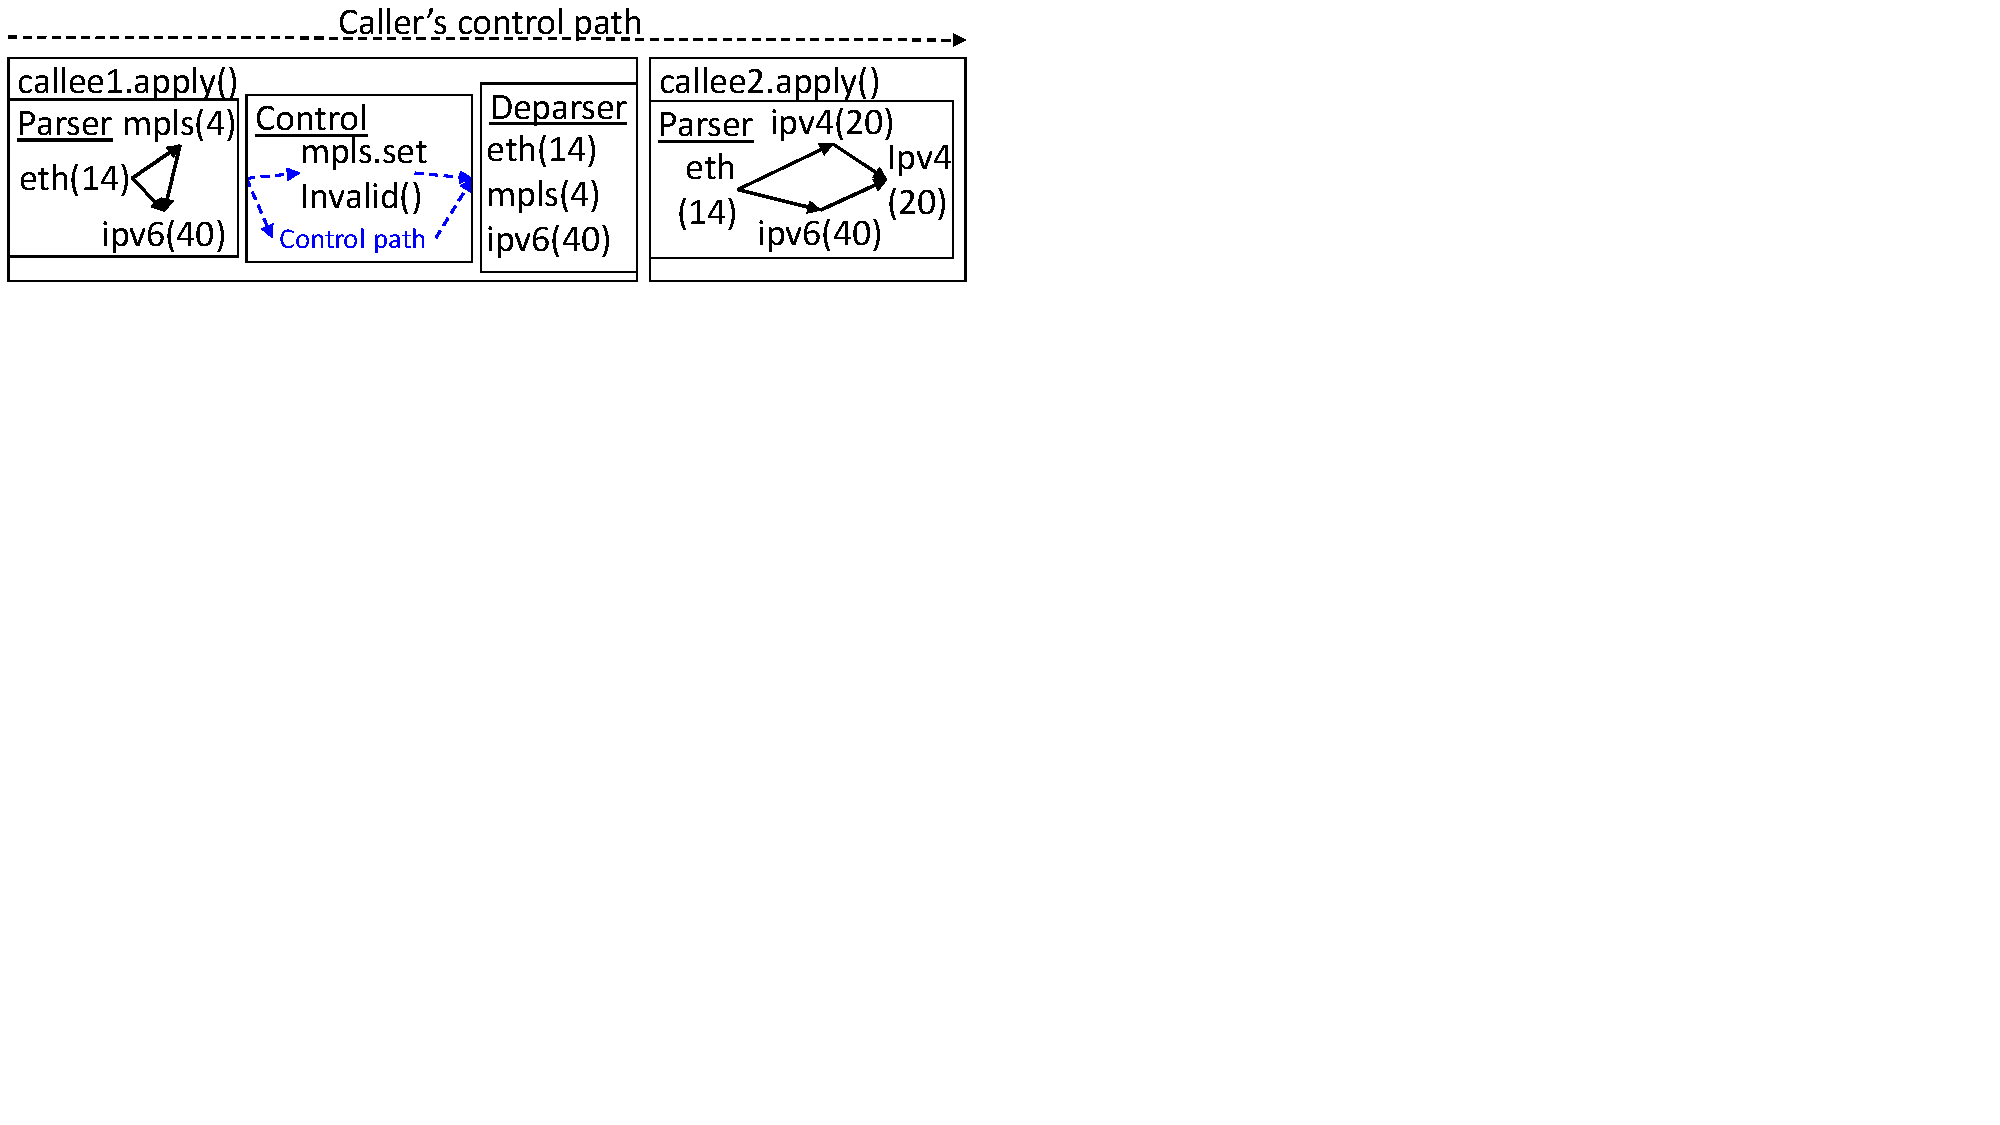
\includegraphics[trim=0 396 487 0, clip,scale=0.5]{sequential-callees}
    \caption{Multiple callees in a control path}
    \label{fig:sequential-callees}
\end{figure}
The $i$\textsuperscript{th} callee may decrease a packet's
size---e.g., a control path of \texttt{callee1} removes the
\texttt{mpls} header, decreasing the size by 4
bytes.  \texttt{callee2} extracts \texttt{eth}, \texttt{ipv4} and
\texttt{ipv6} headers from the packet. So, to
process
\begin{enumerate*}[label=(\roman*)]
  \item removal of 4-byte \texttt{mpls} header by \texttt{callee1} and
  \item extraction of maximum bytes (74-byte \texttt{eth-IPv4-IPv6})
    in \texttt{callee2}'s parser,
\end{enumerate*}
78(=4+74) bytes are required.  So, we take into account the
extract-length of every callee's parser along with the maximum
decrease in packet size by the callee's predecessors in the control
path $x$ to compute $lc_{a}(x)$, as shown in
\cref{extract-length-control-path}.
\begin{align}
lc_{a}(x) \; =& \; \max_{cp} \left\{ \left( \sum_{i=0}^{i<cp} \delta(i) \right)+ El(cp) \right\},&cp \in [0,N] \label{extract-length-control-path} \\
\mathcal{B}s_{a} \; =& \; El(a) + \Delta(a) & \label{byte-stack-size-package}
\end{align}
Finally, we compute the byte-stack size for a \uprogram $a$,
$\mathcal{B}s_{a}$  as the sum of its extract-length and maximum
increase in packet size as shown in \cref{byte-stack-size-package}.
For the example in \cref{fig:sequential-callees}, the byte-stack size
for the caller is 98 ($El$(\texttt{callee2}) =78, and 20 for increase
in \texttt{callee1}) bytes.
% 20 bytes (due to ipv4.setValid()) in addition of its extract-length.
We perform a similar analysis for \textit{min-packet-size}. But, we
skip the details for brevity.
% dthe minimum number of bytes required to extract a packet.
% by the caller's parser or among every possible first callee's parser.

\subsubsection{Parser and Deparser To Match-Action Tables}
\label{subsection:parser-to-match-action-table}
\begin{figure*}[!tb]
    \begin{subfigure}[b]{0.25\linewidth}
        \centering
        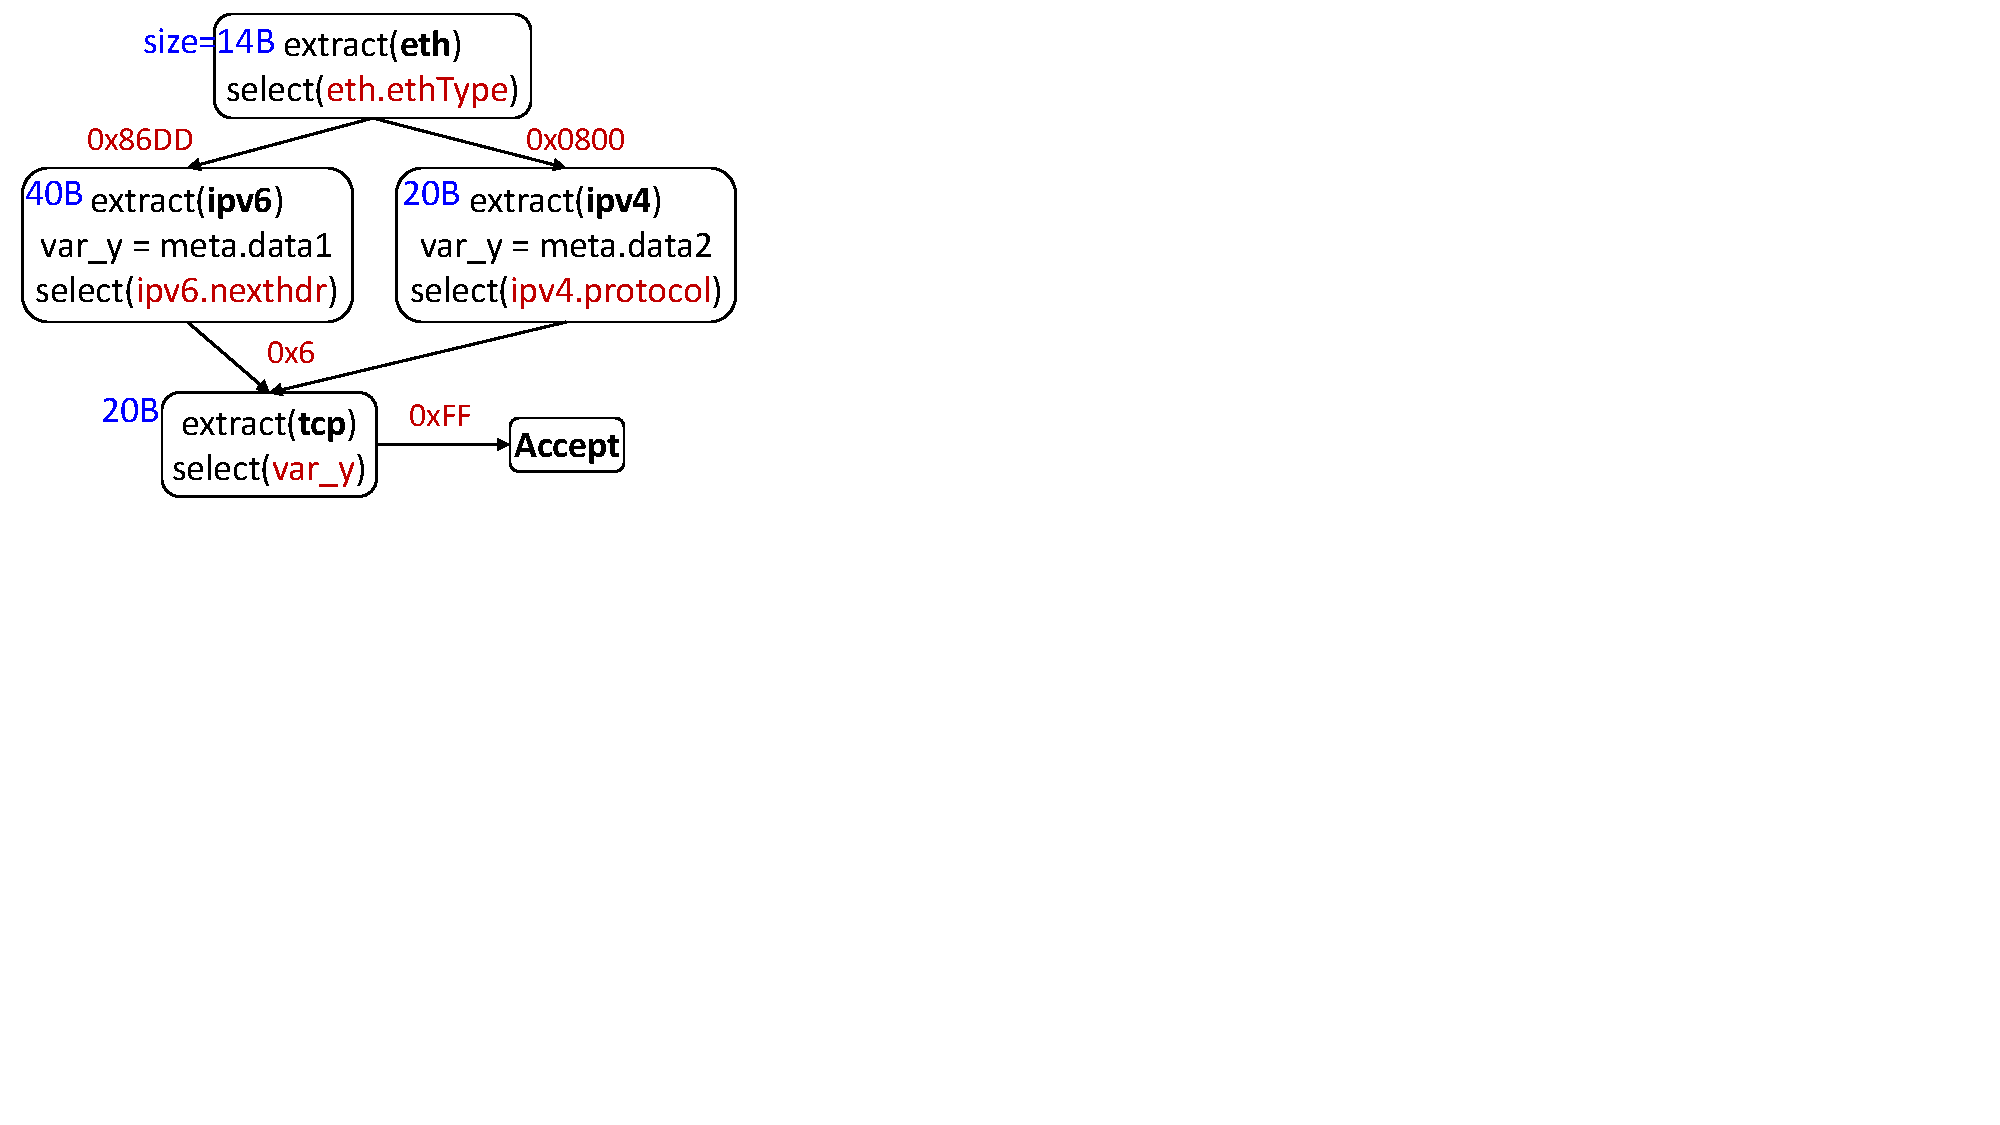
\includegraphics[trim=4 270 596 0, clip,scale=0.37]{parser-transformation-example}    
        \caption{An example P4 parser}
        \label{subfig:parser}
    \end{subfigure}
    \begin{subfigure}[b]{0.26\linewidth}
        \centering
        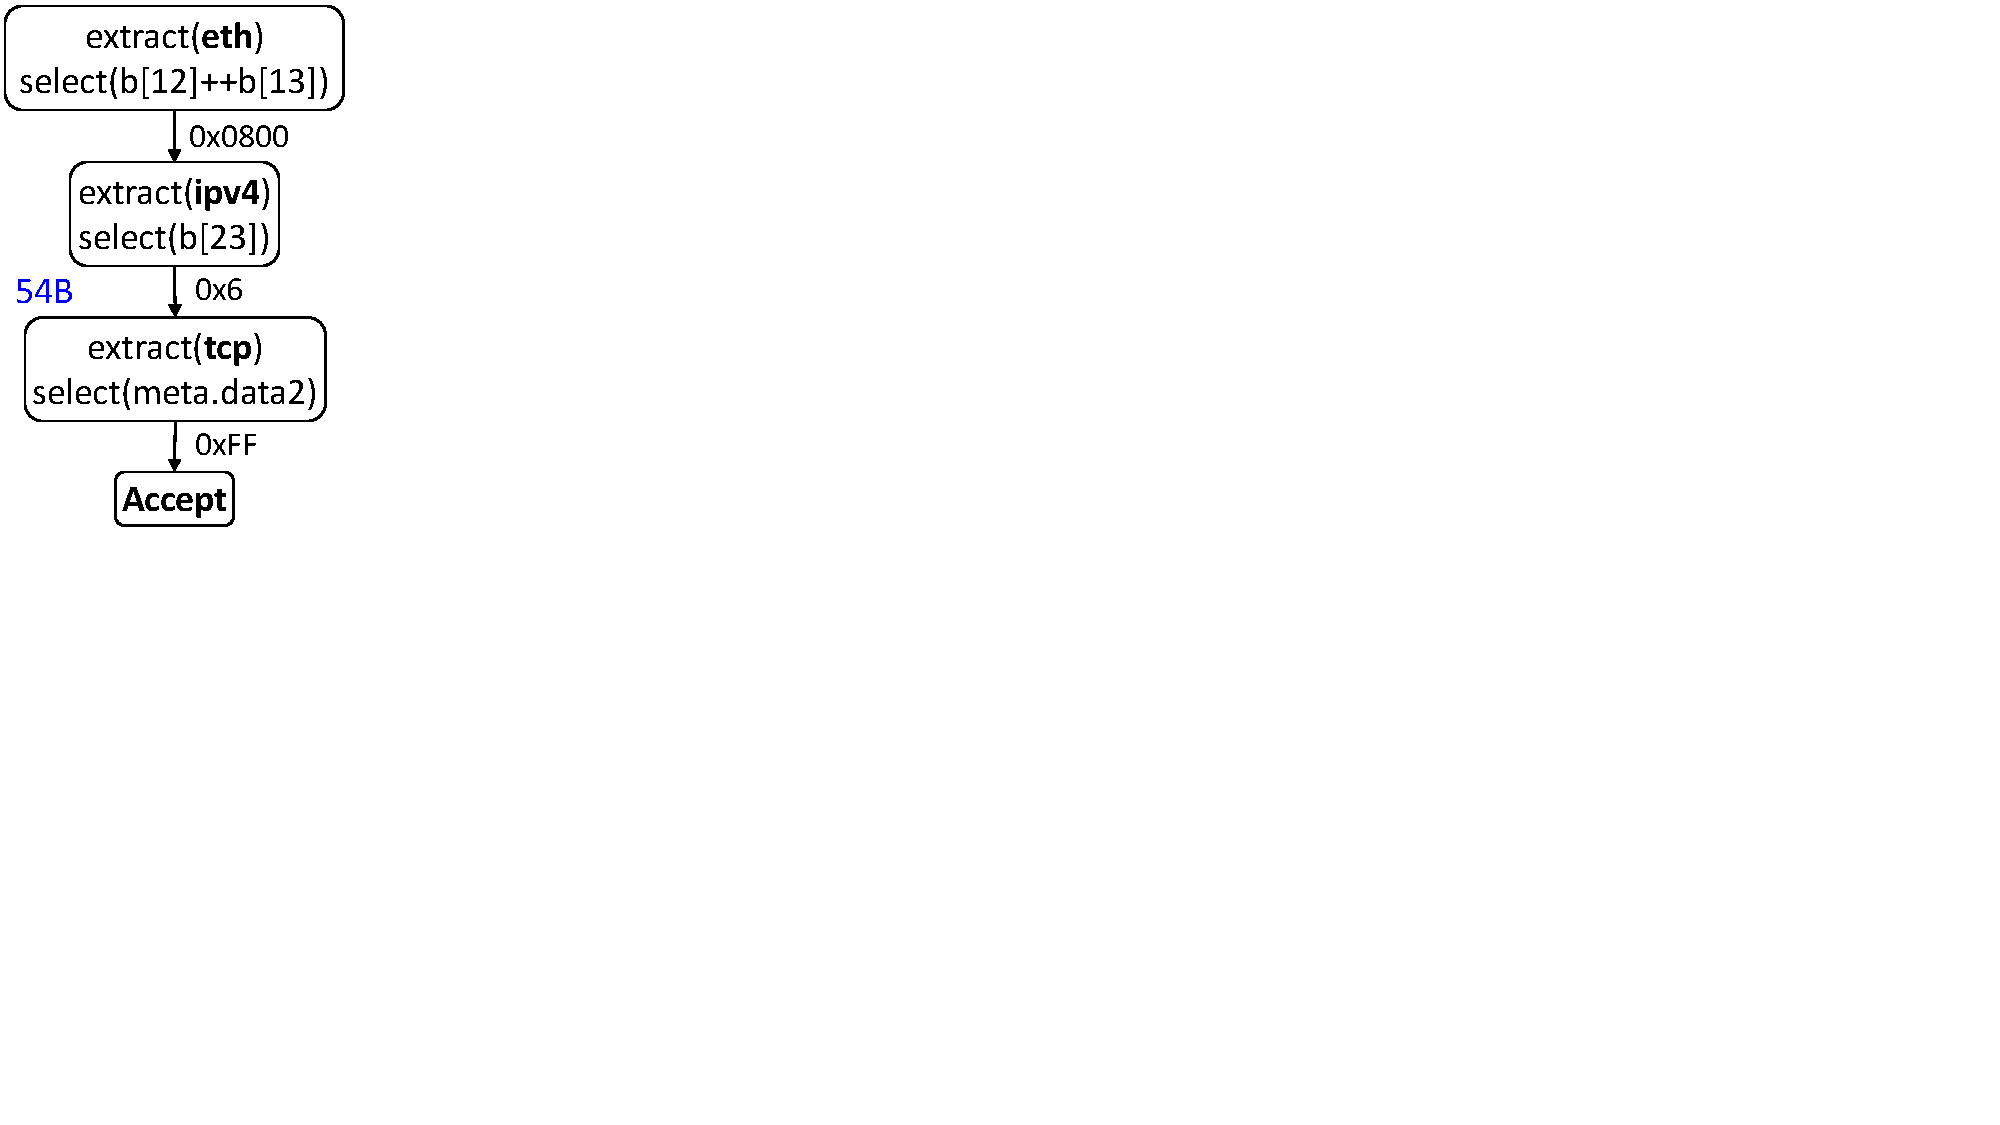
\includegraphics[trim=0 285 794 0, clip,scale=0.37]{parser-example-se-1}
        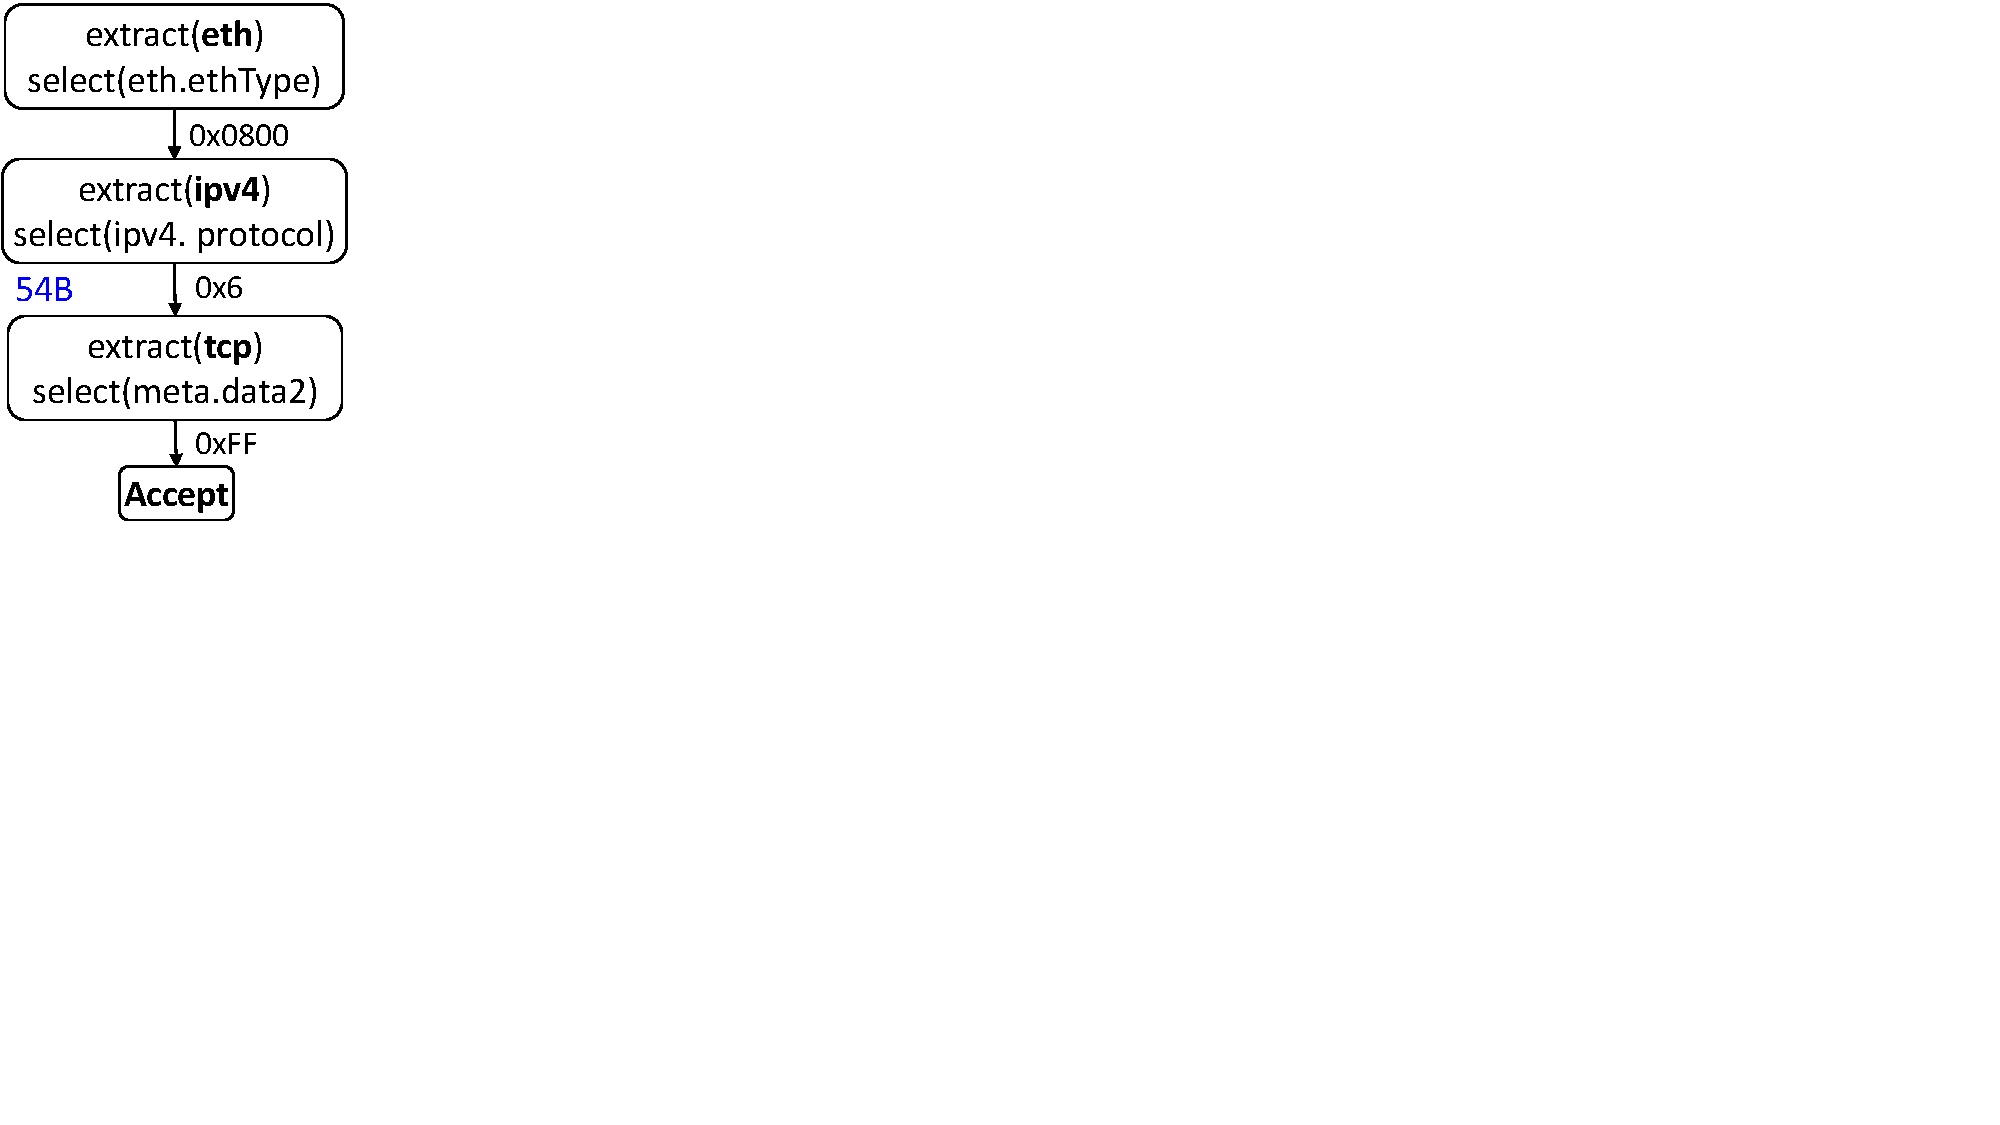
\includegraphics[trim=0 285 794 0, clip,scale=0.37]{parser-example-se-2}
        \caption{Symbolic execution of the parser}
        \label{subfig:parser-symbolic-execution}
    \end{subfigure}
    \begin{subfigure}[b]{.47\linewidth}
    \centering
    \begin{lstlisting}[frame=none, escapechar=!]
key = { !\color{parser-red}{b[12]++b[13]}!:exact; // rest Ternary
  !\color{parser-red}{b[20]}!; !\color{parser-red}{b[23]}!; !\color{parser-red}{meta.data1}!; !\color{parser-red}{meta.data2}!;
  b[53].isValid(); b[73].isValid();}
actions = { cp_eth_ipv4_tcp;
  cp_eth_ipv6_tcp; set_parser_error;}
const entries = {
  (!\color{parser-green}{x0800}!,_,!\color{parser-green}{x6}!,_,!\color{parser-green}{xFF}!,1,_):cp_eth_ipv4_tcp();
  (!\color{parser-green}{x86DD}!,!\color{parser-green}{x6}!,_,!\color{parser-green}{xFF}!,_,_,1):cp_eth_ipv6_tcp();
}
default_action : set_parser_error();
\end{lstlisting}
\vspace*{-10pt}
\caption{Parser converted to match-action control}
\label{subfig:parser-mat}
\end{subfigure}
\caption{Example illustrating parser to control block transformation
by \ucomp.}
\label{fig:parser-to-control-block-transformation}
\end{figure*}

% P4 parser blocks describe parse graphs as state machines. Real 
% target devices contain programmable parser module that can be 
% programmed using parse graphs. 
\tightparbf{Parser.}%
A close look at the design of programmable parsers reveals that they
essentially perform repeated match-action operations~\cite{6665172}.
% Programmable parsers \cite{6665172} are implemented as finite state 
% machines (FSM) using buffer, Ternary Content-Addressable Memories 
% (TCAM) and Action RAM. TCAM matches and processes actions and copy 
% packet header state by  state. Once thecurrent state fields have been 
% matched the next state is identified and the state header bytes are 
% copied.  
% Network packets are of finite length, hence they can be parsed in a 
% finite number of ways. Successful parsing of a packet is essentially 
% finding a match for a finite number of bytes from a finite set of 
% values. Every state path identifies possible byte locations to match 
% for extracting a set of headers instances. We leverage match 
% capability of TCAM in match-action stages to match simultaneously all 
% possible byte locations pertaining to every path from start to the 
% accept state. The final executed action associated with the matched 
% entry copies values from the appropriate locations in the byte-stack 
% to local metadata synthesized for used header fields. In general, we 
% consider that parser state may use any metadata or variable  to 
% transit to the next state see Figure 
% \ref{subfig:parser-symbolic-execution}. 
So, with the operational-region in byte-stack ($b$), we can perform
these operations simultaneously in hardware. We use the parser in
\cref{subfig:parser} as a running example to explain how we synthesize
tables for a parser.

The parser's FSM has four states to extract Ethernet, IPv4, IPv6 and
TCP headers of size 14, 20, 40 and 20 bytes, respectively.  \ucomp
performs symbolic execution of the parser to identify two possibles
paths from the start state to the accept state. Then, it replaces the
header fields in each path---e.g., \texttt{eth.ethType} and
\texttt{ipv6.nexthdr}---with their evaluated offsets in the
byte-stack---e.g., \texttt{b[12]++b[13]} and \texttt{b[23]}---as shown
in \cref{subfig:parser-symbolic-execution}.  It also performs
\emph{Forward Substitution} \cite{Padua:1986:ACO:7902.7904} on every
path to eliminate any anti-dependency between two states---e.g.,
\texttt{var\_y} is replaced with \texttt{meta.data1} in one and
\texttt{meta.data2} in the other.
\deleted{corresponding locations in the byte-stack}
% As an example, \emph{tcp} state transits to the accept state based 
% on value (0xFF) of \texttt{var\_y} variable which is updated by 
% either \emph{ipv4} or \emph{ipv6} states. If the select expression 
% depends on local variables, it performs Forward Substitution 
% \cite{Padua:1986:ACO:7902.7904} on every path to eliminate data 
% dependency. Figure \ref{subfig:parser-symbolic-execution} shows 
% evaluated parser states and two paths generated by symbolic execution 
% with forward substitution. Every extract method-call statement is 
% transformed into assignments from the byte-stack to field-variables 
% associated with the header instance passed as an argument to the 
% method-call.In addition, valid metadata variable pertaining to the 
% header instance is set.

\ucomp creates a match-action entry for each path as follows. Using
the byte-stack offsets and variables used in \texttt{select}
expressions of states in each path
(\cref{subfig:parser-symbolic-execution}), \ucomp synthesizes a
match-key by merging them (\cref{subfig:parser-mat}). To ensure that a packet is long enough to be parsed, the key
also contains validity test for the last byte extracted on the
path. Then, it synthesizes an action for each path---e.g.,
\texttt{cp\_eth\_ipv4\_tcp}---which has assignment statements to copy
the relevant header fields. \ucomp pairs a key with the
appropriate action to create an entry for the path---e.g., in the first entry in \cref{subfig:parser-mat},
\texttt{x0800}, \texttt{x6} \& \texttt{xFF} are matched to the first, third and fifth keys to
parse a byte-stack as ethernet, IPv4 and TCP headers while the
the second and fourth keys are don't care values.

Finally, the midend also converts header fields in each \uprogram to
necessary metadata, called \emph{field-variables}, which is copied
from the byte-stack in the synthesised actions. The field-variables
also include validity flags for headers.
% by using the case fields values to match the path select keys and
% the other remaining fields are set to don't care values.

% \subsubsection{Deparser To Match-Action Table:}
% \label{subsection:deparser-to-match-action-table}

% The deparser blocks of \uarch's pipelines are the control blocks 
% with emitter as one of the parameters. \ucomp replaces the 
% \texttt{emitter} instance's \texttt{emit} method-call 
% statements with match-action table to transform deparser into 
% normal match-action control blocks.
% The match-action table copies back field-variables to appropriate 
% locations in byte-stack based on values of valid metadata variables 
% associated with header instances. 
% The control block of the pipeline may set or reset validity 
% of header 
% instances and, thereby, modifying the size of the packet.
% In case of increase in packet size, byte-stack is always 
% large enough 
% to hold new headers.
% If a deparser decreases the packet size, subsequent parsers may set 
% \texttt{packet\_too\_short} error only if packet-length on the 
% wireis less than the extract-length and greater than the 
% min-packet-size for % the main package.


% The midend transforms the deparser of the program to a 
% match-action table that copies back fields variables to byte-stack.
% The match-action table copies back field-variables to appropriate 
% locations in byte-stack based on values of valid metadata variables 
% associated with header instances.
% The symbolic execution of a deparser derives the emit order of header 
% instances in the block.
% Using the size of header instances and the emit order, we compute 
% offsets in byte-stack to copy back field-variables and to insert new 
% header fields.
% The match key comprises valid metadata variables associated with each 
% header instance in the package.
% For every possible combination of valid headers, we synthesize a 
% series of operations on byte-stack as an action to copy 
% field-variables and to move data in byte-stack.
\tightparbf{Deparser.}%
Using the emit order of header instances and number of bytes extracted
by the parser, \ucomp synthesizes match-key and actions to copy back
field-variables at appropriate offsets in the byte-stack. A \uprogram
may set a header instance (in)valid, thereby, modifying a packet's
size.  In case of an increase, the byte-stack is large enough to hold
new headers. To show the case with decrease, consider \texttt{callee1}
in \cref{fig:sequential-callees}, which invalidates the \texttt{mpls}
header if execution follows a specific control path. Recall that the
synthesized parser extracts 78 bytes in the stack. If execution
follows the path invalidating \texttt{mpls} header, the following 60
bytes, carrying data, are moved up by an offset of 4 in the stack. The
synthesized action performs in-place copy of these 60 bytes and
invalidates the last 4 bytes.
% If the control block execution sets ipv4 header instance to valid, 
% bytes after the ipv6 header are pushed down by the offset of 20 to 
% insert ipv4 header instance.
Finally, the midend removes all user-defined headers local to a
\uprogram.

% The select expression in transition statement could be a header field, metadata or local variable declared in the parser.
% The value of select expression of a state may depend on its ancestors' parser statements. <<as shown in diagram>>
% Therefore, we perform Forward Substitution on select expressions in evaluated instances of states
% % (https://dl.acm.org/citation.cfm?id=7904)
% on each path and eliminate such data dependency.

% We synthesise local binary variables, called \emph{visit},  for each parser state to track the state transition of the parser's FSM.
% For every evaluated instance of a parser state, we synthesise an action comprising its parser\-Statements and replace extract method call statements to assignment statements.
% The assignment statements copies bytes from the buffer array to header instances' fields according to their sizes.
% Next, we add pop method call with the header size as the argument to remove the header from the byte array.
% We insert setValid method call statement for the extracted header instances.
% We add an assignment statement to set visit variable associated with the parser state.


\subsubsection{Preprocessing for \ucomp-backends}
After homogenizing the processing blocks, \ucomp eliminates any
logical buffers for \uprograms that do not use compile-time replication. If a
\uprogram uses compile-time replication of packet and intrinsic
metadata to express multi-packet processing, \ucomp prepares a
\emph{Packet-Processing Schedule (PPS)} graph for the \uprogram. A
node in a PPS graph denotes the \uprogram's sub-program, called
\texttt{thread}, that processes a single packet instance, while an
edge represents dependency among threads. To prepare a PPS by
extracting sub-programs, we construct a Program Dependence Graph
(PDG)~\cite{Ferrante:1987:PDG:24039.24041} from the \uprogram-IR and
perform \emph{slicing} that is defined based on a variant of
\emph{program slice}~\cite{Weiser:1981:PS:800078.802557}. We define
our slicing criteria based on the semantics of logical externs,
\texttt{pkt}, \texttt{in\_buf} and \texttt{out\_buf}, along with
\texttt{apply} method exposed by \uarch's interfaces. See
\cref{subsubsection:packet-processing-schedule} for more details.





% By the end of the midend passes, \ucomp transforms parser and 
% deparser blocks of every package into match-action control blocks, 
% homogenizing abstract-machine of the main package and realizing 
% transition of execution control across callee packages.
% However, control blocks of the packages still contain  
% \uarch-specificconstructs. Next, we discuss backend of \ucomp that 
% further transforms the control blocks to create a packet-processing 
% program a given target architecture.






\subsection{\ucomp Backend}
\label{subsection:micro-backend}
% The backend of \ucomp transforms \ucomp-IR into the target 
% architecture specific IR by $(1)$ mapping control blocks to 
% target architecture-specific pipeline model, $(2)$ translating 
% intrinsic metdata of \uarch to architecture-specific metadata and 
% $(3)$ generating parser-deparser blocks exposed by the target
% architecture.



\ucomp's backend understands semantics of the pipeline model of the
specified target. It also uses a mapping of metadata from \uarch to
the target architecture and captures any constraints on metadata in
the target. It allocates the control blocks in \uarch-IR while
respecting the constraints to the processing blocks exposed by the
target. During the allocation, it also translates the intrinsic
metadata for the target.

% Finally, it uses metrics computed 
% by \emph{static-analysis} in the midend to synthesise target-specific 
% parser and deparser blocks. 
% To allocate a thread on the target architecture's
% pipeline, \ucomp performs required \emph{partitioning} transformation
% on the thread's PDG.

\tightparbf{Allocation to target architecture.}%
For \uprograms that uses packet-replication, the
backend visits PPS nodes in topological order to simultaneously
allocate thread nodes that are at the same level in the ordering. In
the absence of packet-replication, it allocates packet-processing code
of a single thread. Next, we explain the partitioning for single
thread while using \texttt{v1model} as a reference target architecture.


\ucomp's backend for \texttt{v1model} maintains a FSM with two
states---ingress and egress. The FSM captures constraints on the usage
of \texttt{egress\_spec}, \texttt{egress\_port} and queuing metadata
in the ingress and egress blocks. Each state represents a set of
assertions to be verified on visit of every program statement in the
Control Flow Graph (CFG) of the thread---e.g., to prevent accessing
dequeue timestamp of a packet in ingress pipeline, the graph traversal
asserts that every visited statement is NOT a \texttt{im\_t}'s
\texttt{get\_value} method call whose argument maps to
\texttt{v1model}'s intrinsic metadata for deq\_timestamp.  If an
assertion associated with a state fails, the program statement is
marked and not visited. State transition occurs when graph
traversal can not continue due to absence of unmarked and
unvisited nodes. At this point, \ucomp creates two sub-graphs of the
thread CFG---one having visited and the other having unvisited program
statements. The FSM also transits to egress state. Similary, in the egress
state, the graph can enforce egress-specific constraints.
% visited statement is not a method call of \texttt{get\_egress\_port} in \texttt{im\_t} object.
% We perform trivial translation of method calls of \uarch's extern with corresponding method calls of target architecture.

For handling data dependency---e.g., sharing live local
variables,---\ucomp synthesizes \emph{partition-metadata} that can be
passsed as user-metadata between ingress and egress control blocks.
% and live variables to restore execution state.
Nodes across sub-graphs may be connected by edges to represent control
dependencies among sub-graphs. \ucomp converts control dependencies into data
dependencies by synthesizing more metadata.
% Finally, {copy\_from} method calls of \texttt{pkt} instances are 
% replaced for v1model with \texttt{clone3} and \texttt{recirculate} or 
% by synthesizing multicast session while setting appropriate thread-id 
% in user-defined metadata.
% We can perform similar allocations for other architectures using
% appropriate mapping on \texttt{meta\_t} and creating an FSM that
% captures PSA constraints.






% We synthesize \emph{partition} metadata that is assigned a unique value for each control branch in the first partition.
% The second partition uses the metadata and condition on their values to resume execution on appropriate control branch.
% Also, partitioned code may access the same local declaration variables.
% These shared local variables along with the \emph{partition} metadata are passed as user-defined metadata between ingress and egress control block.

% We synthesize per packet user metadata to store thread-id.
% A packet is processed by a thread only if the corresponding thread-id is set in the metadata. 
% We enforce this condition by instrumenting thread code with an if-conditional statement.
% At the end of each thread, next thread-id is set.






%%%%%%%%%%%%%%%%%%%%%%%%%%%%%%%%%%%%%%%%%%%%%%%%%%%%%%%%%%%%%%%%%%%%%%
%%%%% Implementation %%%%%%%%%%%%%%%%%%%%%%%%%%%%%%%%%%%%%%%%%%%%%%%%%
%%%%%%%%%%%%%%%%%%%%%%%%%%%%%%%%%%%%%%%%%%%%%%%%%%%%%%%%%%%%%%%%%%%%%%

\section{Implementation}
\label{sec:implementation}
We have implemented \ucomp by extending the open-source P4 reference
compiler, \texttt{p4c}~\cite{p4c}. In addition to frontend extensions
for \ulang's syntax, \ucomp's midend and backend comprise
\textasciitilde 6,000 LoCs. As supporting a target requires an
architecture-specific backend, our prototype includes a backend for
\texttt{v1model}~\cite{v1model.p4}. To support other targets, \ucomp's
can be extended with the corresponding backend. We have made our
implementation available under an open-source
license\footnote{\url{https://github.com/anonymized-for-review}}.

In the rest of this section, we focus on:
\begin{enumerate*}[label=(\roman*)]
  \item the differences with P4 (\cref{sec:comparison}),
  \item supporting new targets in \ucomp (\cref{sec:new-target}),
  \item the overheads (\cref{sec:overheads}) and
  \item limitations of \ulang (\cref{sec:limitations}).
\end{enumerate*}


\subsection{Comparison with P4}
\label{sec:comparison}
One of our goals is to keep the changes to P4-16 syntax and grammar
minimal so that users familiar with P4-16 can easily adopt \ulang. We
briefly describe these differences. First, \ulang allows defining
custom package types that hide the implementation of a
packet-processing and exposing an interface to reuse the code. Second,
\uarch defines interfaces to encapsulate a set of programmable blocks
so that the logical dataplane pipeline can be extended. Third, \uarch
uses explicit information passing between modules in contrast to
implicit global sharing of metadata in P4.  Finally, instead of using
target-specific constructs, programmers use logical \uarch constructs.
Apart from these, \ulang conforms to the semantics of other P4-16
constructs such as externs, control, parser blocks, etc.

\deleted{Essentially, package types are associated runtime behavior,
unlike P4-16's specification. ... (\texttt{pkt}, \texttt{extractor}
and \texttt{emitter}) compared to ones defined in P4 core library
(\texttt{packet\_in} and \texttt{packet\_out}).}





\subsection{Supporting New Target Architectures}
\label{sec:new-target}
\deleted{\ucomp's frontend and midend translate \ulang programs into
\uarch IR and perform certain optimizations. They do not perform any
target-specific translations.} \ucomp's  backend
(\cref{subsection:micro-backend}) is the only target-specific
component as it translates \uarch-IR into a P4 program for a
specified target. As it maps metadata of \uarch to that of the target,
it needs target architecture-specific mappings for metadata and
methods corresponding to \texttt{meta\_t}, \texttt{im\_t} and
\texttt{mc\_engine} for translation. The backend transformation needs
to conform to the pipeline model declared of the target. Further, if
the midend of the target's compiler is available, \ucomp's backend can
pass the IR to target compiler's midend to generate executable for the
target. Thus, to support a new target, we need to provide \ucomp's
backend with a mapping from \uarch's logical constructs to
target-specific constructs. Our implementation provides an example of
how to do this for \texttt{v1model}.


\subsection{Discussion on Resource Utilization}
\label{sec:overheads}
While \ulang focuses on developing abstractions and compiler
techniques to enable target-agnostic reuse of programs, the
transformation to target-specific configuration may introduce resource
overheads. We discuss some of the possible sources of overheads and
opportunities for optimization.

\subsubsection{Resources in Re-configurable Switches}
\ucomp performs static analysis of \ulang programs to estimate the
size of byte-stack needed (\cref{subsubsection:static-analysis}) and 
synthesizes
a (de)parser to extract/emit bytes from the packet
(\cref{subsection:parser-to-match-action-table}). It transforms
user-defined (de)parser into a match-action table executed in
hardware. We discuss its overhead on two crucial resources in
RMT-based devices:


\tightparbf{1. Packet Header Vector (PHV).} PHV stores parsed headers,
metadata and other data in the pipeline. The size of \ulang byte-stack
impacts PHV consumption in the same way as the size of parsed headers
of monolithic P4 programs. As these remain in scope and live through
all hardware stages, we term such utilization of PHV as \emph{global
usage}. Variables and user-defined metadata used within a control
block also consume PHV, but may not live and consume PHV at all
hardware stages. We term such utilization as \emph{local usage}.

To illustrate and compare global usage, consider the example from
\cref{fig:sequential-callees} and a monolithic P4 version of the
caller, say \texttt{mp}. As \texttt{mp}'s parser is the union of all
parsers, the total size of headers to execute \texttt{mp} would be 98
(for \texttt{eth}+\texttt{mpls}+\texttt{ipv6}+2 \texttt{ipv4}) bytes.
This is the same as that required for \ulang's byte-stack---the
extract-length for the caller is 78, and additional 20 bytes are
required for the ipv4 header set by \texttt{callee1}.  If we consider
the case without \texttt{setValid} and \texttt{setInValid} in
\texttt{callee1}, the required size of byte-stack is $max(54, 74) =
74$. So, in this case, the caller's byte-stack header would have lower
global utilization of PHV compared to \texttt{mp}'s headers. Of
course, this naive analysis considers overheads at the source-level. A
smart target-specific compiler can optimize the PHV needed for
\texttt{mp}, and we believe similar optimizations can be performed for
\ulang. \ucomp, indeed, introduces new local variables within control
blocks.  For example, it removes all header instances and creates
local variables for header fields accessed in control blocks. This may
increase the local utilization of PHV in a hardware stage.

% \ucomp indeed introduces new local variables within control blocks.
% For example, it removes all header instances and creates local
% variables for header fields accessed in control blocks. one stage
% combined, global and local, usages exceeds PHV capacity, allocation of
% match-action tables to hardware stages would play significant role in
% fitting composed program on pipeline.  Our current implementation of
% \ucomp translates to v1model architecture for \texttt{simple\_switch}
% target.
% As a part of future work, we will analyze these two aspects, global and local, PHV consumption for real hardware like Tofino \cite{tofino}.


\tightparbf{2. Number of hardware stages.}%
RMT-based devices have limited number of pipeline stages for
match-action tables while \ucomp's transformations add an extra table
for each (de)parser. As multiple tables can fit in a single stage, and
each new table is relatively small, the overhead on resources is
modest but requires careful placement of
tables~\cite{jose2015compiling}.

Further, \ucomp greatly simplifies the complexity of (de)parser
circuits in hardware as \ucomp accepts all packet with size greater
than min-packet-size and extract bytes up to extract-length estimated
by static-analysis. In fact, this can be implemented with a simple
simple counter-based design.

% However, as the parser consumes only 1-2\% of chip-area, the gain may not be significant to trade for usage of match-action stages in hardware pipeline. 
% Therefore, further optimization would be required to reduce consumption of match-action stages.\\

\tightpar{Optimization.} In cases described in
\cref{subsection:composing-dataplane-programs-of-NFs}, execution of
the match-action table of transformed deparser is followed by another
transformed-parser. As these tables contain static entries, creating a
single table based on their cross-product can reduce the overhead on
match-action stages.




% \subsubsection{Compilation Time}
% We are yet to test \ucomp on extensive set of programs and in composition scenario to conclude on compilation time.
% However, the selective symbolic-execution results in well-know path explosion problem for programs with high branching factor.
% Hence, \ucomp's compile-time analysis can result in significantly huge compilation time.\\
% \textbf{Optimization:}
% We only evaluate method calls of header types, extractor and emitter during symbolic-executable allowing to spawn lightweight threads for parallel execution.
% Further, the computations for extract-length and byte-stack size of \uprograms are highly recursively, therefore they can be avoided by storing and reusing the values during compilation with libraries.





\subsection{Limitations}
\label{sec:limitations}
While \ulang enables us to achieve our goals of portable, modular and
composable dataplane programming, our current implementation of \ucomp
has certain limitations. These limitations do not affect modularity
and composability, but slightly limit the portability of dataplane
programs.

\tightparbf{Stateful memories.}
Many applications require stateful processing of packets. To support
these, architectures provide various constructs to maintain state in
the dataplane---e.g., PSA provides counters, meters and registers.
Currently, \uarch doesn't provide a portable abstraction for such
constructs. So, while a \ulang program can still use these constructs
for stateful packet processing, it cannot be ported automatically
across architectures which differ in these constructs.

\tightparbf{Switch CPU-dataplane interface.}
\uarch does not provide a generic abstraction for communication
between the dataplane and the switch CPU. To use such functionality,
programmers have to use target-specific constructs such as
\texttt{digest} and \texttt{packet\_in} for PSA.

\tightparbf{Device capabilities.}
Target devices support match-action tables with a fixed set of match
capabilities---such as exact, LPM, ternary, and range. \ulang requires
a target to support all match kinds used in a program and \ucomp does
not transform across different match kinds as it requires translating
table entries at runtime. For example, translating a range match entry
for a target that supports only exact match requires enumerating the
range at runtime, while our focus is on compile-time abstractions.
Similarly, \ulang cannot automatically synthesize implementations for
new checksum computations, action selector, and action profiles.

% There exist unified mechanism and abstraction (Control Plane APIs) to configurable data plane from control plane.
% However, data plane program still lacks an abstract to send data or packets to control plane.
% For example, PSA constructs two different, digest and packet\_in, constructs to send data to control plane.
% There could be more higher-level abstraction that can be translated to either of them.

%% The common practice is to expose varying types of constructs in architecture of the target for stateful packet-processing.
%% For example, PSA provides counters, meters and registers for stateful packet-processing.
%% % Again, such constructs for stateful packet-processing hinders portability.
%% \uarch does not abstract away such stateful constructs and exposes them to programmers.
%% However, it could be feasible to automatically allocate stateful data in program to appropriate type of memory available on device.
%% Compilers of Most programming languages analyze scope and lifetime of variables to allocate them on appropriate type of memory.
%% Currently, \ucomp does not perform any such analysis and relies on specific constructs included in \uarch, limiting portability on targets with different constructs for stateful memory.
%% 
%% The lifetime and scope of such state also varies with applications.





\section{Evaluation}
\label{sec:evaluation}
To test the expressiveness and composability of \ulang, we have
implemented a set of applications in \ulang. We present a subset of
these to illustrate some novel ways in which  we can compose \ulang
programs to build real applications.

\subsection{Composing Packet-Processing Layers}
\label{subsection:composing-packet-processing-layers}
Packets are structured into layers of protocols headers with specific
layouts, where each layer is specialized for a specific role.  So,
writing modules for processing one or more layers is a natural way to
build applications as these modules can be developed incrementally,
composed together, and reused.
\tightparbf{Layered Modularity.}
\uarch's generic interfaces allows programmers to define custom
interfaces for modules to exchange data. These can be used to compose
\ulang modules for different network layers. To demonstrate this, we
built a modular router by composing together independent modules
responsible for processing each layer. For example,
\cref{fig:modular-router} shows how we can compose modules for
processing the L2 (Ethernet) and and L3 (IPv4) headers.
% Figure \ref{fig:incremental-development} shows an example of incremental development, which adds SRH processing to support SRv6 in the network.
% \begin{figure}[!h]
% \begin{subfigure}[b]{\linewidth}
%  \begin{lstlisting}[frame=none]
% // srv6.p4
% header ext_routing_h { ... }; 
% header srh_h { ... }; header ipv6_h { ... }; 
% struct srv_ht { 
%   ipv6_h ipv6; ext_routing_h er; srh_h sr;
% };
% parser P(extractor e, pkt p, out srv_ht h) {
%   state start {
%     e.extract(p, h.ipv6);
%     transition select (h.ipv6.nextHdr) {
%       0x2B : parse_routing_hdr; }
%   }
%   state parse_routing_hdr { ... }
%   state parse_srh { ... }
% }
% control C(pkt p, inout srv_ht h, im_t im) {
%   apply { // copy next segment address from h.sr to h.ipv6.destAddr}
% }
% control D(emitter em, pkt p, in srv_ht h) {
%   apply { 
%     em.emit(p, h.ipv6);
%     em.emit(p, h.er); em.emit(p, h.sr);
%   }
% }
% \end{lstlisting}
% \caption{\texttt{srv6} \uprogram to support IPv6 SRH\cite{srh}}
% \label{subfig:srv6}
% \end{subfigure}
% \begin{subfigure}[b]{\linewidth}
% \begin{lstlisting}[frame=none, escapechar=!]
% 0x86DD : { 
%   !\colorbox{mygray}{srv6\_i.apply(p, sm, es);}!
%   ipv6_i.apply(p, sm, es, h);
% }
% \end{lstlisting}
% \caption{Extending \texttt{router} \uprogram}
% \label{subfig:extending-modular-router}
% \end{subfigure}
% \caption{Incremental Development}
% \label{fig:incremental-development}
% \end{figure}


\tightparbf{Incremental Development.}%
For the same program, suppose we want to replace IP routing with
another approach based on segment routing (SRv6). With \ulang, one can
independently and incrementally develop another module for segment
routing, say \texttt{srv6}, to process IPv6 Segment Routing
Header~\cite{srh}. And, we can reuse this module in our modular router
from \cref{subfig:router-main} as follows:

\begin{lstlisting}[frame=none, escapechar=!]
0x86DD : {
  !\colorbox{mygray}{srv6\_i.apply(p, im, h);}! // copies next segment address from SRH header's list to IPv6's destAddr field
  ipv6_i.apply(p, im, h);
}
\end{lstlisting}
The snippets shows how we can integrate SRv6 without touching any
other module used in the router.




\subsection{Composing Network Functions (NFs)}
\label{subsection:composing-dataplane-programs-of-NFs}
Many network functions (NFs) such as firewall and intrusion detection
process complete packets across protocol layers. Operators often need
to deploy such programs on devices using various combinations as per
some policy. To enable this, prior work on dataplane composition, such
as P4Bricks~\cite{soni:hal-01632431} and
P4Visor~\cite{Zheng:2018:PLV:3281411.3281436}, and virtualization,
such as HyPer4~\cite{Hancock:2016:HUP:2999572.2999607} and
HyperV~\cite{8038396}, define operators based on certain use cases.
\ulang naturally supports such composition using a combination of
\ulang-specific features such as user-defined package types and native
P4 constructs such as conditionals.

\tightparbf{Composition Operators.}%
The following \ulang snippet shows an example of how one can express
\emph{sequential} and \emph{override} composition operators from
CoVisor~\cite{188954}.
% \begin{lstlisting}[frame=none, escapechar=!]
% // Sequential: Firewall -> Routing
% firewall.apply(p, sm, es);
% if (sm.drop == false) {
  % // Override: Routing decision
  % elephant_flow_routing.apply(p, sm, es);
  % if (sm.drop == true) 
    % modular_router.apply(p, sm, es);
% }
% p4_int.apply(p, sm, es);
% \end{lstlisting}
\begin{lstlisting}[frame=none, escapechar=!]
// Sequential: Firewall -> Routing -> INT
firewall.apply(p, im);
if (im.drop == false) {
  modular_router.apply(p, im);
  // Override: routing decision
  elephant_flow_routing.apply(p, im);
}
p4_int.apply(p, im);
\end{lstlisting}
First, a packet is processed by the \texttt{firewall} module, which
may decide to drop it after analysing one or more headers. Otherwise,
the packet is routed.  While routing, \texttt{elephant\_flow\_routing}
may override normal routing if the packet belongs to a large flow.
Finally, \texttt{p4\_int} updates the INT (In-band Network Telemetry)
\cite{Kim2015InbandNT, p4int} header with the appropriate data. Note
that even though \uarch does not have a notion of ingress and egress
pipelines, it declares intrinsic metadata which can be mapped to INT
data at the appropriate location in target pipeline. For example,
\emph{ingress timestamp} of INT is mapped to \ulang's
\texttt{IN\_TIMESTAMP}. When compiling for a target such as
\texttt{v1model}, \ucomp partitions the composed pipeline and
allocates \texttt{p4\_int} to the egress pipeline.

Another interesting example of composition is the \texttt{A-B Testing}
operator defined in P4Visor\cite{Zheng:2018:PLV:3281411.3281436}.
\ulang can implement it as follows:
\begin{lstlisting}[frame=none, escapechar=!]
/* A-B Testing in core devices*/
// parser extracts 1 byte header with flag
extractor.extract(p, testHdr);
// Inside control block, the `p` w/o testHdr
if (h.testHdr.testFlag == 1)
  test_prog.apply(p, im);
else
  prod_prog.apply(p, im)
// deparser puts back the test header
emiiter.emit(p, testHdr);
\end{lstlisting}






\subsection{Advanced Processing}
Many applications---e.g., mirroring~\cite{rasley2014planck},
statistics collector such as NetFlow and
sFlow~\cite{panchen2001inmon}, packet history based telemetry as in
NetSight~\cite{179783}, and differential
testing~\cite{Zheng:2018:PLV:3281411.3281436}---require selectively
creating copies of packets and processing the copies in different
manners. \ulang enables such processing through
\texttt{Orchestration}, \texttt{copy\_from} method in \texttt{pkt},
and \texttt{im} externs. The following snippet illustrates creating a
copy of a packet \texttt{pk} and differential processing.
\begin{lstlisting}[frame=none]
struct e_t {}; // empty type
sflow(pkt, im_t);// sFlow implements Unicast
control con(pkt pk, im_t md, 
    out_buf<e_t> ob) { // `ob' holds out packets
  pkt pk2;  im_t md2;
  in_buf<e_t> ib; // in_buffer for another module
  apply {
    pk2.copy_from(pk); // copying
    md2.copy_from(md); // copying
    sflow.apply(pk2, md2); // sflow on copy
    ob.enqueue(pk, md); // puting original in ob
    ob.enqueue(pk2, md2); // copy in ob
    ob.to_in_buf(ib); // moves all elements to ib
    modular_router_orch.apply(ib, ob);
  }
} // inside an Orchestration pipeline
\end{lstlisting}
The \texttt{sflow} module processes a copy of the packet and metadata.
Then, the original packet as well as the processed copy are queued
into an output buffer \texttt{ob}. \texttt{to\_in\_buf} moves the
contents of \texttt{ob} to another buffer, \texttt{ib}, and resets
\texttt{ob}. Finally, the \texttt{modular\_router\_orch} routes
packets between modules.






\subsection{Experience Composing \uprograms}
We implemented a library of independent packet-processing functions in
\ulang to test its expressiveness. To reuse these, we composed a
subset in various ways to build new dataplane applications as shown in
\cref{tab:loc-of-composed}. Each row corresponds to a module, and each
column corresponds to a dataplane generated by composing the modules
for checked rows.
The bottom row shows the line of P4 code generated in the output of
\ucomp when building the dataplane for  v1model~\cite{v1model.p4}
architecture of BMv2 target.
% The huge number of lines, even for two \uprograms, is a result of
% byte-level match-action tables generated by \ucomp.


\begin{table}[!htp]
\begin{center}
\begin{tabular}{|c|c|c|c|c|c|c|}
  \hline
  \textbf{\ulang programs} & \multicolumn{6}{|c|}{\textbf{Composed dataplane}} \\ 
\hline
  L2 & \checkmark & \checkmark & \checkmark & \checkmark & \checkmark 
& \checkmark  \\ \hline
  IPv4 & \checkmark &  & \checkmark & \checkmark &  \checkmark & 
\checkmark  \\ \hline
  IPv6 &  & \checkmark &  &   &  &  \\  \hline
  ECN &  &  & \checkmark &  &  & \checkmark  \\ \hline
  Firewall &  &  &  & \checkmark &  & \checkmark  \\ \hline
  NAT &  &  &  &  & \checkmark & \checkmark \\
  \hline \hline
  \textbf{Target P4 LoC} & 656 & 684 & 879 & 1084 & 1068 & 1693 \\ \hline 
\end{tabular}
\caption{Composing \ulang programs to build dataplanes. Bottom row
shows LoC in the output of \ucomp for \texttt{v1model} target.}
\label{tab:loc-of-composed}
\end{center}
\end{table}

\section{Related Work}
\label{sec:related-work}
Over the last decade, there has been a great effort in programmable 
networks to compose network policies (Pyretic 
\cite{180291}, NetKat \cite{Anderson:2014:NSF:2535838.2535862} ), 
controllers (Frenetic \cite{2034812}, Corybantic 
\cite{Mogul:2013:CTM:2535771.2535795} Flowbricks \cite{6980389}, 
CoVisor \cite{188954}) and  dataplane (Hyper4 
\cite{Hancock:2016:HUP:2999572.2999607}, HyperV \cite{8038396}, 
P4Visor \cite{Zheng:2018:PLV:3281411.3281436}), 
because, networks are complex to manage and configure 
without having a modular approach.

The work on composing control plane and static policy focus on 
defining a set of composition operators that can be used to describe 
packet-processing policies without incurring race-conditions and 
inconsistencies. This approach suits to control plane programs as 
each program specifies complete behavior of packets in the network or 
on the device. Inspired form control plane compositions, prior work 
on dataplane composition has focused on defining composition operators 
based on use cases that process every packet in its entirety. Our work 
significantly differs as we enable the fundamental mechanism, invoking 
one dataplane program from another, that allows programmers to reuse 
fine-grained packet-processing code and define custom composition 
operators. Reuse of dataplane program poses challenge of 
portability. In this aspect, our framework is orthogonal to PSA 
\cite{psa}. PSA exposes a dataplane model that target device 
must realise. Instead, we focus on abstraction that programmers can 
use to write portable dataplane programs. \ucomp framework is inline 
with Domino \cite{Sivaraman:2016:PTH:2934872.2934900} that 
provides abstractions to describe stateful algorithm with reference 
to its Banzai model and compiles them to target-specific 
low-level microcode.

Conceptually, the design of \uarch resembles more with the Click 
Modular Router\cite{Kohler:2000:CMR:354871.354874} than PSA. The 
Click allows to compose packet processing modules, called 
\emph{elements}, that can be connected together using \emph{push} or 
\emph{pull} ports to create a directed graph. The edges of the 
graph determines flows of the packets. Our approach slightly differs 
here, \uarch's interfaces allows to transfer the control and data 
along with packet. Also, the Click is software framework that is 
targeted for general purpose compute machines, whereas \ulang 
framework targets RMT based devices.


\section{Conclusion}
Dataplane programs are evolving to be complex and diverse with novel
use cases, such as those arising from in-network compute, and we are
also starting to see a variety of target devices. So, we believe that
the programming model must facilitate writing portable, modular and
composable programs. To support this, we introduce \ulang which raises
the level of abstraction from target-specific packet-processing
pipelines and constructs. With \ulang, users can write
target-agnostic, self-contained modules independently, and compose
them to build larger programs while supporting a range of devices.



\clearpage
%-------------------------------------------------------------------------------
\bibliographystyle{plain}
\bibliography{main}


\appendix
\section{Declarations in \uarch}
\label{appendix:section:micro-switch-architecture}
We describe exact declarations of \texttt{Unicast}, 
\texttt{Multicast} and \texttt{Orchestration} interfaces along with 
their runtime behavior. 

% \begin{figure*}[h]
% \begin{minipage}[t]{.35\textwidth}
% \begin{lstlisting}[frame=none]
% extern pkt {
%   byte[] packet;
%   unsigned length;
%   void copy_from(pkt p);
% }
% extern emitter {
%   void emit<H>(pkt p, in H hdr);
% }
% \end{lstlisting}
% \end{minipage}\vline
% \hfill\begin{minipage}[t]{.22\textwidth}
% \begin{lstlisting}[frame=none]
% enum meta_t {
%   INGRESS_TIMESTAMP,
%   EGRESS_TIMESTAMP
% }
% struct sm_t {
%   bit<16> pkt_len;
%   bit<8> in_port;
% }
% \end{lstlisting}
% \end{minipage}\vline
% \hfill\begin{minipage}[t]{.41\textwidth}
% \begin{lstlisting}[frame=none]
% extern mc_engine {
%   mc_engine();
%   void set_mc_group(GroupId_t gid);
%   apply(es_t, out PacketInstanceId_t);
%   
%   set_buf(out_buf<O>);
%   apply(pkt, es_t, out O);  
% }
% \end{lstlisting}
% \end{minipage}
% \begin{minipage}[t]{0.40\textwidth}
% \begin{lstlisting}[frame=none]
% extern extractor {
%   void extract<H>(pkt p, out H hdr);
%   void extract<H>(pkt p, out H hdr, in bit<32> size);
%   H lookahead<H>();
% }
% extern es_t {
%   void set_out_port(in bit<8>);
%   bit<8> get_out_port();
%   bit<32> get_value(in meta_t ft);
%   void copy_from(im_t im);
% }
% \end{lstlisting}
% \end{minipage}\vline
% \hfill\noindent\begin{minipage}[t]{0.57\textwidth}
% \begin{lstlisting}[frame=none]
% extern in_buf<I> { // used only by architecture
%   dequeue(pkt, es_t, out I);
% }
% extern out_buf<O> {
%   enqueue(pkt p, im_t im, in O out_args);
%   void to_in_buf(in_buf<O>);
%   void merge(out_buf<O>);
% }
% extern mc_buf<H, O> {
%   enqueue(pkt, in H, es_t, in O);
% }
% extern void recirculate();
% \end{lstlisting}
% \end{minipage}
% \end{figure*}


% \begin{figure}[h]
% \begin{lstlisting}[frame=none]
% extern pkt {
%   // byte array representation
%   byte[] packet;
%   unsigned length;
%   void copy_from(pkt p);
% }
% extern emitter {
%   void emit<H>(pkt p, in H hdr);
% }
% extern extractor {
%   void extract<H>(pkt p, out H hdr);
%   void extract<H>(pkt p, out H hdr, in bit<32> size);
%   /// H may be an arbitrary fixed-size type.
%   H lookahead<H>();
% }
% \end{lstlisting}
% \caption{Packet Representation}
% \label{fig:pkt-externs}
% \end{figure}

% \begin{figure}[h]
% \begin{lstlisting}[frame=none]
% enum meta_t {
%   INGRESS_TIMESTAMP,
%   EGRESS_TIMESTAMP
% }
% extern es_t {
%   void set_out_port(in bit<8>);
%   bit<8> get_out_port();
%   bit<32> get_value(in meta_t ft);
%   void copy_from(im_t im);
% }
% \end{lstlisting}
% \caption{\texttt{es\_t} extern}
% \label{fig:msa-egress-spec-extern}
% \end{figure}
% 
% \begin{figure}[h]
% \begin{lstlisting}[frame=none]
% extern in_buf<I> {
%   // used by architecture only
%   dequeue(pkt, es_t, out I);
% }
% extern out_buf<O> {
%   enqueue(pkt p, im_t im, in O out_args);
%   void to_in_buf(in_buf<O>);
%   void merge(out_buf<O>);
% }
% extern mc_buf<H, O> {
%   enqueue(pkt, in H, es_t, in O);
% }
% \end{lstlisting}
% \caption{Buffer Representation}
% \label{fig:pkt-buf}
% \end{figure}
% dequeue(pkt, out H, es_t, out O);

% \begin{figure}[h]
% \begin{lstlisting}[frame=none]
% // This can only be used in control block of multicast interface
% extern mc_engine {
%   mc_engine();
%   void set_mc_group(GroupId_t gid);
%   apply(es_t, out PacketInstanceId_t);
%   
%   set_buf(out_buf<O>);
%   apply(pkt, es_t, out O);  
% }
% \end{lstlisting}
% \caption{Multicast Extern}
% \label{fig:msa-multicast-extern}
% \end{figure}



% \begin{figure}[h]
% \begin{lstlisting}[frame=none, escapechar=!]
% struct out_t { /* empty */ }
% control mc(pkt p, hdr_t h, sm_t s, es_t e, !\colorbox{mygray}{mc\_buf<hdr\_t, out\_t> hb}!) {
%   !\colorbox{mygray}{mc\_engine mce;}!  PktInstId_t id; 
%   out_t  oa;
%   action replicate(GroupId_t gid) {
%     !\colorbox{mygray}{mce.set\_mc\_group(gid);}!
%   }
%   table MulticastRouting{
%     key = { h.ipv4.dstAddr : exact; } 
%     actions = { replicate; }
%   }
%   table mac{
%     key = { es.get_port() : exact; } 
%     actions = { mac_update; }
%   }
%   apply {
%     MulticastRouting.apply();
%     !\colorbox{mygray}{mce.apply(es, id);}!//similar to C's fork
%     mac.apply();
%     hb.enqueue(h, sm, im, oa);
%   }
% }
% \end{lstlisting}
% \caption{Multicast Example}
% \label{fig:multicast-example}
% \end{figure}

\begin{figure*}[h]
\begin{lstlisting}[frame=none]
// Unicast
Unicast<H,M,I,O,IO>(pkt p, im_t im, in I in_param, out O out_param, inout IO inout_param) {
  parser u_parser(extractor ex, pkt p, out H hdr, inout M meta, in I in_param, inout IO inout_param);
  control u_control(pkt p, inout H hdr, inout M m, im_t im, in I in_param, out O out_param, inout IO inout_param);
  control u_deparser(emitter em, pkt p, in H hdr);                             
}

// Multicast
Multicast<H,M,I,O>(pkt p, im_t im, in I in_param, out_buf<O> ob) {
  parser m_parser(extractor ex, pkt p, out H hdr, inout M meta, in I in_param);
  control m_control(pkt p, inout H hdr, inout M meta, im_t im, inout I in_param, mc_buf<H,O> mob);
  control m_deparser(emitter em, pkt p, in H hdr);
}

Orchestration<I,O>(in_buf<I> ib, out_buf<O> ob) {                         
  control o_control(pkt p, im_t im, in I in_param, out_buf<O> ob);
}    
\end{lstlisting}
\caption{Interfaces declares in \uarch}
\label{fig:programmable-blocks-for-interfaces}
\end{figure*}








\section{Multicast extern}
\label{app:multicast}
\begin{lstlisting}[frame=none, escapechar=!]
control mc(pkt p, hdr_t h, im_t im,
    !\colorbox{mygray}{mc\_buf<hdr\_t, out\_t> hb}!) {
  !\colorbox{mygray}{mc\_engine mce;}!  PktInstId_t id; 
  !\colorbox{mygray}{out\_t oa;}! // some out args
  action replicate(GroupId_t gid) {
    !\colorbox{mygray}{mce.set\_mc\_group(gid);}!
  }
  table MulticastRouting{ key = { ... } 
    actions = { replicate; }
  }
  table mac{ ...}
  apply {
    MulticastRouting.apply();
    !\colorbox{mygray}{mce.apply(im, id);}!//similar to C's fork
    mac.apply();
    !\colorbox{mygray}{hb.enqueue(h, im, oa);}!
  }
}
\end{lstlisting}
The two arguments to \texttt{apply} pass required information
(\texttt{im\_t} and \texttt{PktInstId\_t}) for each replica. The first
argument provides an instance of \texttt{im\_t} having out port
already set for the replica of the packet.  The second argument having
\texttt{out} direction provides packet instance id to identify the
replica.

The methods \texttt{set\_buf} and \texttt{apply (pkt, im\_t, out O)}
facilitate nested invocation of \upackages with multicast interface.
Programmers can use \texttt{set\_mc\_group} method in actions or apply
blocks to set a replication group for the packet.




\section{\ucomp Midend Transformations}

\subsection{Header Stack Transformation}
\label{subsection:header-stack-transformation}
\ulang allows to use of header stacks with their size known at 
compile-time. 
\ucomp replaces every header stack instance with multiple instances of 
the header type. 
It symbolically evaluates operations on the header stack instances and 
transforms them into appropriate built-in method calls of the 
instances.
P4 provides various sets of computations to use in parser and control 
blocks.
In parser blocks, programmers can use \texttt{next} and \texttt{last} 
operations to iterate through the stack.
These operations along with \texttt{lastIndex} can be used to write 
loops in parsers to extract instances in header stack.
\ucomp unrolls such loops by replicating the parse states in them.
Loop unrolling replaces relative referencing operations, \texttt{next} 
and \texttt{last}, with appropriate header instances in the state 
replicas.
P4 provides \texttt{push\_front} and \texttt{pop\_front} operations on 
stack instances to manipulate elements on top and bottom of the stack.
\ucomp transforms push\_front and pop\_front operations into series of 
assignments and built-in method calls of header instances.
For example, assume that \texttt{hs} is a header stack instance of 
size 3. 
\ucomp synthesize hs0, hs1, hs2 header instances to replace hs.
\texttt{hs\_inst.push\_front(1)} is replaced with \texttt{hs2 = hs1}, 
\texttt{hs1 = hs0} and \texttt{hs0.setInvalid()}.


\subsection{Header Stack Transformation}
\label{subsection:header-stack-transformation}
\ulang allows programmers to define variable-length header types, 
however it imposes a constraint that their variable-length fields must 
contain integer number of bytes at run-time.
\ucomp splits header type containing fixed and variable-length 
fields into multiple types, where each type contains either 
fixed-length fields or the variable-length field.
\ucomp transforms every parser state with two-argument extract method 
call, used to extract variable-length header, into a sub-parser.
It splits the header type of the instance in the first argument into 
multiple header types, where each type contains either fixed-length 
fields or 
the variable-length field.
Every state in the sub-parser extracts a fixed-number of bytes from 
the packet byte stream.
The sub-parser contains a state having the second argument 
(variableFieldSize) as the expression in its select statement.
The select statement has case-list enumerating all possible values up 
to specified maximum size of the variable-length field.
For each select case, the sub-parser transits to a state extracting a 
fixed number of bytes in the variable-length field.
For example, if variable-length field has maximum size of 40 bytes, 
\ucomp creates 40 states extracting different number of bytes.
The explosion of number of states would only increase number of 
entries in the transformed match-action table of the parser.

% \begin{figure}[H]
% \begin{minipage}[c]{0.45\linewidth}
% \begin{lstlisting}[frame=none]
% header_t[3] hs;
% 
% hs.push_front(1);
% \end{lstlisting}
% \end{minipage}
% \begin{minipage}[c]{0.45\linewidth}
% \begin{lstlisting}[frame=none]
% header_t hs0, hs1, hs2;
% 
% hs2 = hs1;
% hs1 = hs0;
% hs0.setInvalid()
% \end{lstlisting}
% \end{minipage}
% \caption{Extern to }
% \label{fig:}
% \end{figure}





\subsection{Packet-Processing Schedule}
\label{subsubsection:packet-processing-schedule}


\begin{figure}[!h]
\begin{lstlisting}[frame=none]
struct e_t {};  struct h_t { ... };
prog(pkt, im_t, out h_t);
test(pkt, im_t, out h_t);
log(pkt, im_t, in h_t, in h_t);
control validate(pkt p, im_t i, out_buf<e_t> ob) {
          pkt pt, pm;  im_t it, im;  
/*slice*/ h_t hp, ht;
/*  #  */ apply {
/*  1  */   pm.copy_from(p); // c1
/*  1  */   im.copy_from(i);
/*  3  */   pt.copy_from(p); // c3 
/*  3  */   it.copy_from(i);
/* 2,1 */   prog.apply(p, i, hp); 
/* 3,1 */   test.apply(pt, it, ht); 
/*  1  */   if (hp != ht) {
/*  1  */     log.apply(pm, im, hp, ht);
/*  1  */     ob.enqueue(pm, im);
/*  1  */   }
/*  3  */   im.set_out_port(DROP);
/*  2  */   ob.enqueue(p, i);
/*  3  */   ob.enqueue(pt, it);
          }
       }
\end{lstlisting}
\caption{Multi-Packet Processing}
\label{fig:multi-packet-processing}
\end{figure}





If the main package has callees with orchestration interface, \ucomp 
extracts packet-processing threads and PPS for control block of every callee.
\ucomp constructs a Program Dependence Graph(PDG) 
\cite{Ferrante:1987:PDG:24039.24041} having statements as nodes and 
dependencies among them as edges. \ucomp  performs a series of transformations on PDG to compute PPS.


% \ucomp treats parameter of orchestration control block or every \texttt{copy\_from} method call statement of \texttt{pkt} instance as its definition, because they initialize the instance.
% We note that \texttt{pkt} instance argument in \texttt{copy\_from} method calls is only used or read.
% Moreover, all other method call statements having \texttt{pkt} instances as arguments access (read and modify) the instances, such call statements are not considered as their definition statements.
% We define \emph{access-ranges} of a \texttt{pkt} instance's definition as span of program statements until the next definition of the instance in reached on every possible path in the PDG.

For every initialization statement of a \texttt{pkt} instance, we 
define an \emph{access-range}, analogous to live ranges, as span of 
program statements until the next initialize of the instance in 
reached on every possible path in the PDG.
We merge overlapping access-ranges of multiple initialization of the 
same \texttt{pkt} instance. If an instance has non-overlapping 
access-ranges, a new instance for every access-range is synthesised to 
create one-to-one mapping between them.


Inspired from \emph{program slice} defined in 
\cite{Weiser:1981:PS:800078.802557}, we define \emph{packet slice} 
based on access-ranges. A packet slice of a \texttt{pkt} instance is 
an executable subset of PDG, which consists of all the program 
statements affecting the instance's value in its access-ranges.
A set of initialization statements of \emph{pkt} instance with 
overlapping access-ranges is considered as a slicing criteria for a 
given packet instance. Packet slices can have multiple entry and 
exist points due to presence of conditional statements.
We compute packet slices from the PDG of control block using a method 
similar to one described in \cite{Ferrante:1987:PDG:24039.24041}.
Specifically, we perform a graph traversal in reverse direction of 
edges from every statement at exit points in the access-ranges until 
initialization statements in the criteria are reached.
The graph traversal continues until all possible definitions of every 
variable used in visited statement are reached.
If any variable or extern instance is involved in anti-dependency, it 
is resolved by introducing new variable and renaming.
An example program shown in \cref{fig:multi-packet-processing} 
is sliced with respect to definitions of three instances 
\texttt{pm}, \texttt{p} and \texttt{pt}.


Packet slices of different instances may have common program 
statements due to control and data dependencies. Therefore, a packet 
slice may have method call statements processing different \emph{pkt} 
instances than one's initialization statements used in slicing 
criteria. For the program shown in \cref{fig:multi-packet-processing}, 
slice 1 pertaining to instance \texttt{pm} shares program statements 
with slices 2 and 3 related to \texttt{p} and \texttt{pt}, 
respectively.
We create a packet-processing thread per instance by excluding such 
method call statements from every packet slice but maintain dependency 
among them by creating inter-thread dependency.
% All other common program statements not accessing \texttt{pkt}
% instances are also excluded from threads.
All other common program statements are also excluded from threads of 
\texttt{pkt} instances. We term such statements \emph{cps} nodes and 
maintain their control and data dependencies with the thread nodes.
% We associate every thread with an identifier, \emph{thread-id}, and 
% a set of group-ids, called \emph{clone-group}.
We associate every thread with an identifier, \emph{thread-id}, and 
synthesize metadata for it. \ucomp synthesizes if-conditional 
statement in every thread to execute its program statements only if 
its id value is set in thread-id metadata.

\deleted{
Every thread-id identifies a thread based on unique \texttt{pkt} 
instance processed by it. In presence of conditional statements, a 
thread may process a packet copied from one of multiple possible 
packet instances. Every group-id identifies set of threads that may 
process copies of the same packet instance.
}


% and clone-group identifies every possible \texttt{pkt} instances from which the thread's packet instance could be initialized.

We follow similar approach to extract threads associated with \texttt{in\_buf} instance.
The \texttt{merge} and \texttt{to\_in\_buf} methods of \texttt{out\_buf} easily allows to add thread nodes and control dependency among them in PPS.

We transform PDG to PPS graph by coalescing all the nodes in a thread to a single node while maintaining their control and data dependencies with cps and other thread nodes.
We synthesise a variable to transform every control dependency among thread nodes to a data dependency.
The thread, which is depended on, sets the variable with a constant value and the other thread uses the variable in predicate of new if-conditional statement to continue processing on the control path.
If a PPS has a directed cycle involving thread nodes, PPS is not serializable.
If the target architecture does not have capability to process multiple copy of a packet at the same time,
\ucomp raises error and lists program statements involved in cycles.
However, a PPS can have cycles involving maximum one thread node and cps nodes.
To decide execution thread for cps nodes, we compute strongly connected components of PPS graph.
In each component, there can be exactly one thread node and one or more cps nodes.
We further transform PPS into a DAG by coalescing cps nodes in a component to its thread node.
PPS can still have cps nodes not part of any SCC, such nodes can be executed as a part of any thread.
We schedule such cps nodes while mapping the thread components to data plane of target architecture.

% Every \texttt{apply} method call statement of \texttt{Multicast} or \texttt{Orchestration} type package gets transformed to a thread node in PPS.
% \texttt{enqueue}, \texttt{merge} and \texttt{to\_in\_buf} method call statements of \texttt{out\_buf} extern's instances capture dependence among such threads nodes in PPS.

%%%%%%%%%%%%%%%%%%%%%%%%%%%%%%%%%%%%%%%%%%%%%%%%%%%%%%%%%%%%%%%%%%%%%%%%%%%%%%%%
\end{document}
%%%%%%%%%%%%%%%%%%%%%%%%%%%%%%%%%%%%%%%%%%%%%%%%%%%%%%%%%%%%%%%%%%%%%%%%%%%%%%%%

%%  LocalWords:  endnotes includegraphics fread ptr nobj noindent
%%  LocalWords:  pdflatex acks
